% ============================================================
%  SLOWLAB — workshop / conference submission
%  Compiles directly on Overleaf (pdfLaTeX). Depends on no external .sty file.
%
%  To switch to a conference template: replace the \documentclass and geometry
%  settings below with \usepackage{neurips_2026} (or the relevant template); nothing
%  in sections/ needs to change.
% ============================================================
\documentclass[10pt]{article}

\usepackage[margin=1in]{geometry}
\usepackage[utf8]{inputenc}
\usepackage[T1]{fontenc}
\usepackage[expansion=false]{microtype}  % expansion=false only for compatibility with some TeX distributions; can be dropped on Overleaf
\usepackage{amsmath,amssymb,amsthm}
\newtheorem{definition}{Definition}
\usepackage{graphicx}
\usepackage{booktabs}
\providecommand{\euro}{\texteuro}
\usepackage{multirow}
\usepackage[table]{xcolor}
\usepackage{caption}
\usepackage{subcaption}
\usepackage[hidelinks]{hyperref}
\usepackage{url}
\usepackage{natbib}
\usepackage{enumitem}
\usepackage{titlesec}
% ---- Colours for the code highlighting in Figure 2 (light background, print-friendly;
% a dark background is too loud inside the body text) ----
\definecolor{cKw}{RGB}{0,86,160}      % keywords
\definecolor{cCls}{RGB}{128,64,160}   % class names
\definecolor{cFn}{RGB}{20,125,85}     % method names
\definecolor{cStr}{RGB}{170,50,50}    % strings
\definecolor{cCmt}{RGB}{120,120,120}  % comments
\newcommand{\pykw}[1]{\textcolor{cKw}{\bfseries #1}}
\newcommand{\pycls}[1]{\textcolor{cCls}{\bfseries #1}}
\newcommand{\pyfn}[1]{\textcolor{cFn}{#1}}
\newcommand{\pystr}[1]{\textcolor{cStr}{#1}}
\newcommand{\pycmt}[1]{\textcolor{cCmt}{\itshape #1}}

\usepackage{tikz}
\usetikzlibrary{tikzmark,arrows.meta,calc}
\usepackage{placeins}
\renewcommand{\topfraction}{0.92}
\renewcommand{\textfraction}{0.06}
\renewcommand{\floatpagefraction}{0.80}
\setcounter{topnumber}{2}
\raggedbottom   % allow slack at the foot of a page rather than an overfull vbox

% ---- Note macro: marks unfinished places while drafting; set \draftmode to false
% before submission ----
\newif\ifdraftmode\draftmodetrue
\newcommand{\todo}[1]{\ifdraftmode{\color{red}\textbf{[TODO: #1]}}\fi}
\newcommand{\pending}[1]{\ifdraftmode{\color{orange}\textbf{[PENDING: #1]}}\fi}

% ---- Notation shorthands ----
\newcommand{\slowlab}{\textsc{SlowLab}}
\newcommand{\Pone}{\textbf{P1}}
\newcommand{\Ptwo}{\textbf{P2}}
\newcommand{\Pthree}{\textbf{P3}}
\newcommand{\Pfour}{\textbf{P4}}

\titlespacing*{\section}{0pt}{1.1em}{0.5em}
\titlespacing*{\subsection}{0pt}{0.8em}{0.35em}

\title{\slowlab: Benchmarking Scientific Agents When Experiments Are\\
Slow, Noisy, Costly, and Irreversible}

\author{
  \todo{authors and affiliations}
}
\date{}

\begin{document}
\maketitle

\providecommand{\pending}[1]{\textcolor{gray}{\textsc{#1}}}
\begin{abstract}
Benchmarks for automated experimental design make experiments instantaneous, free, and
infinitely repeatable. Real experiments are none of these. We introduce \slowlab, an
executable benchmark under four conditions that hold at once: feedback is slow, noise is
irreducible, trials are priced in the objective's own units, and commitments cannot be
rolled back. An agent runs a greenhouse --- it designs experiments, commits them, waits out
a growing cycle, and repeats. Ground truth is a published mechanistic crop model, so the
difficulty is not ours to tune, and everything is denominated in net profit per square metre
per day. Beside realised regret we report the regret a perfect reasoner would still carry
given the same design, computed from an instance distribution no agent sees. The gap
separates a campaign that could not have answered the question from one that could and did
not, and scores an agent against what was achievable rather than against a baseline we
happened to implement.

Across five models and four tasks, $99\%$ of designs on the six-factor screen cannot
separate the effects they were commissioned to separate, because most use two distinct
treatments replicated across the facility: under a hard parallelism cap, precision and
coverage compete for the same physical units. This is the opposite of the failure we
expected. Supplying standard tools then drives the two measures apart --- the designs
improve and the campaigns end worse in sixteen of twenty cells, because the inference
tool is fitted to the agent's own design, inherits its deficiency, and is deferred to in
proportion to how wrong it is. Under these conditions an agent cannot afford the cycle it
would take to find that out.
\end{abstract}

\section{Introduction}
\label{sec:intro}

Language-model agents are increasingly proposed as operators of scientific experimentation:
selecting what to run, interpreting what comes back, and deciding what to run next
\citep{coscientist,chemcrow,szymanski2023autonomous}. The claim attached to this work is
that such agents will accelerate discovery in domains where experiments are the bottleneck.
Whether that claim holds is an empirical question, and answering it requires evaluating
agents under the conditions that make experimentation a bottleneck in the first place.

Existing evaluations do not. In the benchmarks available for automated experimental design,
an experiment is a function call: it returns immediately, costs nothing, and may be repeated
without limit \citep{boxinggym}. Under those conditions the strategy that wins is the one
that queries most, and a poor decision is corrected by making another. Neither property
survives contact with a laboratory. A commercial tomato crop occupies its greenhouse for
seven months and more; a synthesis run consumes reagents and instrument time; a cohort study, once enrolled, cannot be
re-enrolled. In these settings the binding constraint is not the agent's throughput of ideas
but the fact that each idea must be paid for in time and material, and that a design once
committed cannot be revised. An agent optimised against free, instantaneous, repeatable
experiments is being selected on a proxy from which the operative difficulty has been
removed, and we currently have no executable environment in which to find out whether that
selection transfers.

The gap is recognised in the domain literature, which asks for exactly the properties an
idealised environment cannot expose---cost-aware performance, constraint-violation behaviour,
reproducibility (\S\ref{sec:related})---and lacks an environment in which to measure them.

\paragraph{\slowlab.} We introduce an executable benchmark for experimental design under
four conditions that hold at once. Feedback is \textbf{slow}: a cycle is $210$ days, and
the number of trials that run concurrently is capped --- unevenly, because some factors are
set for a whole block of units and others per unit, so replication and coverage compete for
the same physical resource. Observations are \textbf{noisy} enough that one unit does not
settle a question. Experimentation is \textbf{costly} in the objective's own units, since
testing a management regime means growing a crop under it and selling whatever results. And
a submitted design is \textbf{irreversible}: no branch, no checkpoint, no revert. Each
condition alone is familiar. Together they withdraw the recourse every existing benchmark
assumes, because an agent can neither buy precision and coverage from the same units nor
find out which it needed before the season ends.

The conditions define a class rather than a domain --- microbial evolution, bioprocess
scale-up, materials ageing and dose-finding trials satisfy them too, and
Appendix~\ref{app:admit} states what a domain must supply to be admitted. We instantiate
the first in controlled-environment horticulture, where a published mechanistic crop model
\citep{jones1999reduced} coupled to an explicit economic one puts the difficulty outside
our control and every quantity in one currency, net profit per square metre per day
(\S\ref{sec:domain}). The agent's action is a \emph{design}: which factor settings to test,
on how many units, and which physical units those are. Lamps and heating serve a whole
chamber while planting density and the pruning target are set per hydroponic loop, so an
allocation that varies temperature between two loops of one chamber describes an experiment
that cannot be performed. Having committed, the agent sees nothing until the cycle ends;
after two or three cycles it must recommend. Figure~\ref{fig:overview} is the whole loop
on one page.

\begin{figure}[t]
\centering
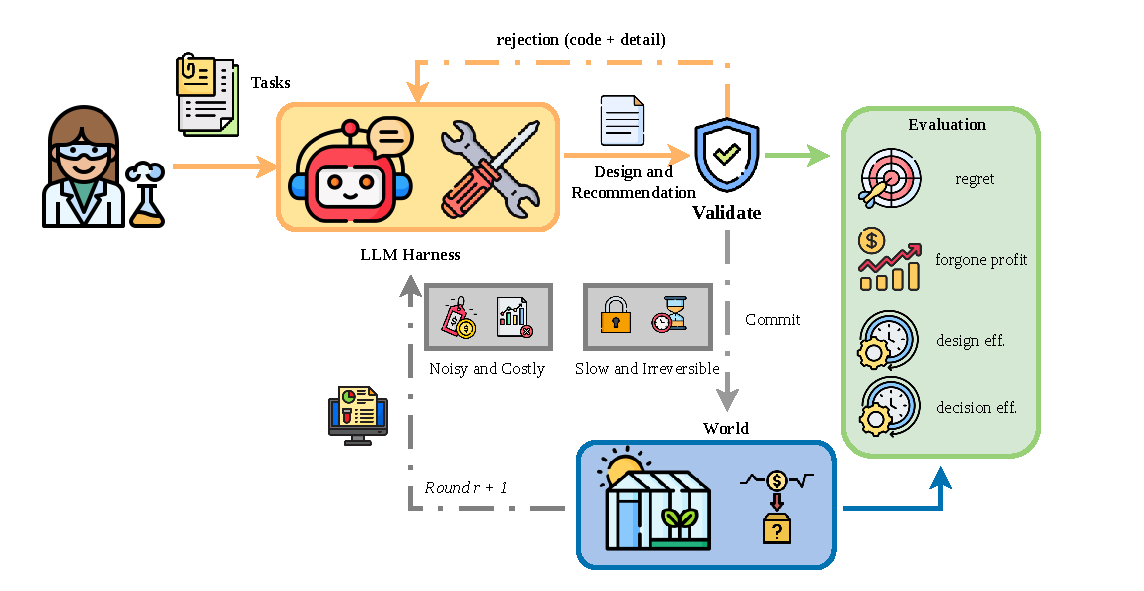
\includegraphics[width=\linewidth]{figures/fig0_overview.pdf}
\caption{\textbf{Overview.} A seed draws a \emph{site}---a parameter vector for the crop
model---from a published between-site spread, unknown to the agent. Each round the harness
serialises the state, the agent returns a complete design and an interim recommendation,
and the design is checked for mechanical feasibility only: a rejection carries a code and a
detail and costs no budget, so the agent may revise without penalty. Committing is the
irreversible step. Committed units are occupied for a full growing cycle---$210$ days, so a
three-round campaign runs for $630$---and the harness returns their values when that cycle
ends. What the agent is denied is not sight of the crop but any action to take on it while
the units are busy. Units are not interchangeable: some factors are set per chamber
and others per loop, so replication and coverage draw on the same physical resource. At the
end the campaign is read three ways: the regret its recommendation realised, the profit its
experiments forwent, and how much of the room its designs closed and its decisions then
used (\S\ref{sec:eval}).}
\label{fig:overview}
\end{figure}

Overall, our work makes the following contributions:
\begin{enumerate}[leftmargin=1.5em,itemsep=3pt,topsep=3pt]
  \item We introduce \slowlab, a \emph{framework for experimental design under slow, noisy,
    costly and irreversible trials}, in which one harness --- protocol, action space,
    feasibility checker, agent interface --- serves a class of domains rather than a single
    one. A domain enters by supplying a published response model, a cost model denominated
    in the objective, and a block structure that makes allocation a decision
    (Appendix~\ref{app:admit}); horticulture is the first, so the optimum is a crop model's
    and not ours to tune.

  \item We introduce a \emph{decision-theoretic measure of design quality}: the regret a
    perfect reasoner would still carry given the design, computed from an instance
    distribution no agent sees. It separates a campaign that could not have answered the
    question from one that could and did not, contains no baseline of ours, and is the
    expected value of sample information --- a batch Knowledge Gradient
    (Appendix~\ref{app:eig}).

  \item We conduct \emph{the first evaluation of language-model agents under these four
    conditions jointly}: five models, four tasks, twenty instances each. We expected
    over-exploration and found the reverse --- most designs use two distinct treatments,
    leaving $99\%$ of six-factor screens unable to separate the effects they were
    commissioned to separate. Supplying a screening tool repairs the designs and makes the
    campaigns end \emph{worse} in sixteen of twenty cells: one intervention, two measures,
    opposite directions.
\end{enumerate}

\section{Related work}
\label{sec:related}

\paragraph{Experimental design benchmarks.} \citet{boxinggym} is the closest prior work.
It scores design quality by expected information gain about the parameter vector---the
Bayesian optimal-experimental-design objective, estimated by nested Monte Carlo. We take
the same stance, that design quality should be measured from theory rather than from a
hand-built checklist. We do not take the same quantity. Ours is a decision-theoretic
one: the Bayes risk a design leaves behind on the \emph{recommendation}, not the entropy it
removes from the parameters (\S\ref{sec:eig}). A design can pin $\theta$ down tightly and
spend its budget far from the optimum, which scores well on theirs and badly on ours; their
task is model discovery and ours is a decision. And the
regime differs: experiments there are instantaneous, free and unboundedly repeatable, with no
parallelism constraint and no irreversibility, so the arithmetic behind our main result---a
replicate and a new treatment competing for the same physical unit---cannot arise.

\paragraph{Optimal experimental design.} The quantity in our second contribution is old.
Bayesian experimental design begins with \citet{lindley1956} and is surveyed by
\citet{chaloner1995}; its decision-theoretic branch, which scores a design by the Bayes
risk it leaves on a \emph{decision} rather than by the entropy it removes from parameters,
is \citet{raiffa1961} and \citet{howard1966}. The same object appears in Bayesian
optimisation as the Knowledge Gradient \citep{frazier2008kg}, beside entropy-search
criteria that target the optimum's location instead \citep{hennig2012,hernandez2014}.
Estimating any of them is the standing difficulty \citep{rainforth2018}, and
Appendix~\ref{app:eig} reports how ours failed before it worked. What we contribute is not
the measure but its use as a benchmark score under conditions --- capped parallelism,
priced trials, no retries --- in which an agent cannot substitute more queries for a better
design.

\paragraph{Task validity.} \citet{spade} trains a model to author
executable environments and solve them in self-play, scoring \emph{task} quality by
hint-based regret, $r_D(e)=\bar r_A(e\mid h)-\bar r_A(e)$: the gain a solver gets from
privileged information. This is a lightweight estimate of the minimax-regret objective of
PAIRED \citep{paired}, with the hint-equipped agent standing in for the antagonist, and it
separates environments at the learning frontier from those already mastered or intractable.
A benchmark needs exactly this, since the alternative is to assert that one's tasks are
well-posed. We report it as a diagnostic rather than adopt it as our score: with four
hand-built configurations we can price a task directly against what a perfect reasoner
could extract from it (\S\ref{sec:eig}), whereas hint regret estimates reachability from a
solver's behaviour, which is what one needs when the environments are generated at scale.
It earned its place by correcting us. \textsc{Screen} is the task we came closest to
withdrawing, since its ceiling sits below the noise a full budget leaves
(Table~\ref{tab:tasks}); it also carries the largest hint gap of the tasks the diagnostic
scores, $0.27$ against $0.15$--$0.17$. A task can be at the frontier of what a solver can
do and still be one where instance-tailoring is worth little, and only one of the two
instruments sees each fact. Note that ``validity'' in that work means executability; the
word is already claimed in this literature for something other than inferential soundness.

\paragraph{Self-driving laboratories.} \citet{sdlsurvey} survey deployed self-driving
laboratories and argue that evaluation should ``prioritise decision quality under
constraints and reproducibility rather than single-number performance in idealised
settings''. They prescribe the reference agents we adopt---``random and space-filling
designs, standard BO for short-horizon tasks''---with the aim of providing ``stable
reference points that reflect decision structure, not to maximise baseline performance''
(Appendix~\ref{app:refs}). What is missing is an executable environment in which any of it can
be measured.

\paragraph{Adjacent benchmarks.} ScienceAgentBench, DiscoveryBench and related suites
\citep{scienceagentbench,discoverybench} evaluate analysis and reproduction of published
findings, where the data already exist and the agent bears no collection cost. WOFOSTGym and CropGym expose crop simulators
as RL \emph{control} problems \citep{wofostgym}---the agent sets irrigation over time rather
than committing to a design and waiting; we reuse the framing but not the task. A
substantial literature builds autonomous laboratories
\citep{szymanski2023autonomous,burger2020mobile,coscientist,chemcrow}, surveyed by
\citet{stach2024sdl} and \citet{abolhasani2023rise}; those systems operate on hour-to-day timescales and report
constraint-violation behaviour rather than releasing an executable benchmark.

\section{\slowlab}
\label{sec:regime}
\label{sec:env}

\subsection{Regime and problem formulation}
\label{sec:conditions}
\label{sec:formulation}

\slowlab{} targets sequential experimental design under four conditions that hold jointly.
\textbf{Slow}: what can be learnt per unit of calendar time is bounded by feedback latency
\emph{and} by a hard ceiling on how many trials run concurrently---a facility with a
thousand chambers and a four-month cycle is not slow in the sense that binds. That ceiling
is \emph{tiered}, because some factors are set for a whole block of units and others per
unit, so replication and coverage compete for the same physical resource.
\textbf{Noisy}: a single unit does not settle a question, which is what turns replication,
blocking and allocation into decisions rather than formalities. \textbf{Costly}: a trial
consumes resources measured in the objective's own units, so exploration is priced rather
than free. \textbf{Irreversible}: a submitted design cannot be rolled back---no branch, no
checkpoint, no revert---so the only remedy for a bad design is a new one in a later cycle,
and the units it occupied are gone. Table~\ref{tab:landscape} places existing evaluation
environments against these conditions. We instantiate the regime in controlled-environment
agriculture (\S\ref{sec:domain}).

\begin{table}[t]
\centering\footnotesize
\setlength{\tabcolsep}{3.5pt}
\begin{tabular}{@{}llccc@{}}
\toprule
& & \textbf{Agent / design} & \textbf{Chemistry \& materials} & \textbf{\slowlab} \\
& & {\scriptsize BoxingGym} & {\scriptsize A-Lab, Coscientist} & {\scriptsize (this work)} \\
\midrule
\multirow{2}{*}{\textbf{Slow}}
  & feedback latency        & seconds--minutes & hours--days & \textbf{210 days} \\
  & parallel width          & unbounded & high (96/384-well) & \textbf{hard-capped, tiered} \\
\addlinespace[2pt]
\textbf{Noisy}
  & signal-to-noise         & deterministic & high & \textbf{low (plant-to-plant)} \\
\addlinespace[2pt]
\multirow{2}{*}{\textbf{Costly}}
  & cost of one trial       & $\approx 0$ & reagents, instrument time & \textbf{a crop, priced in the objective} \\
  & cost of a retry         & $\approx 0$ & low--moderate & \textbf{one growing season} \\
\addlinespace[2pt]
\textbf{Irreversible}
  & can a design be undone? & fully (reset) & largely (re-run) & \textbf{no} \\
\bottomrule
\end{tabular}
\caption{Evaluation environments against the four conditions of \S\ref{sec:regime}. Each row
is one measurable property of the condition naming it. The closest prior benchmark differs
on every row.}
\label{tab:landscape}
\end{table}

\paragraph{Problem formulation.} An instance is a parameter vector $\theta \sim P_\Theta$,
unknown to the agent, determining a response $f_\theta : \mathcal{X} \to \mathbb{R}$ on a
factor space $\mathcal{X} \subseteq \mathbb{R}^{d}$ and measured in the objective's own
units. Over $R$ rounds the agent commits a \emph{design} $D_r \in \mathcal{D}$ --- a finite
set of treatments in $\mathcal{X}$ together with their assignment to the physical trial
slots $\mathcal{U}_r$ --- and states a recommendation $\hat{x}_r \in \mathcal{X}$. The
admissible set $\mathcal{D}$ belongs to the facility rather than to the task;
\S\ref{sec:facility} gives it for our instantiation. Its one structural role here is that it
is not all finite multisets: an agent cannot buy precision and coverage with the same slots.

Committing holds $\mathcal{U}_r$ for a cycle of length $\Delta$, after which each slot
returns one observation
\begin{equation}
  y_u \;=\; f_\theta\!\left(x_u;\, \phi_u\right) \;+\; \varepsilon_u,
  \qquad \varepsilon \sim \mathcal{N}\!\big(0, \Sigma(D_r)\big),
  \label{eq:obs}
\end{equation}
where $x_u$ is the treatment assigned to slot $u$ and $\phi_u$ an independent per-slot draw
of the response model's own parameters. Two features of \eqref{eq:obs} carry \textbf{noisy}.
Drawing $\phi$ per slot rather than adding a scalar error makes the variance heteroscedastic
in $x$ and structured by the mechanism; and $\Sigma(D_r)$ is not diagonal, so \emph{where} a
treatment is placed changes what the round can resolve, not only which treatments were
chosen. Appendix~\ref{app:eig} gives $\Sigma$ for our instantiation.

The other three conditions restrict the action. Writing $\mathcal{F}_r = \sigma\big(\{\,y_u
: u \in \mathcal{U}_1 \cup \cdots \cup \mathcal{U}_{r-1}\,\}\big)$ for everything returned
before round $r$, and $\mathcal{A}_r$ for the entire action set available at round $r$,
\begin{equation}
  D_r,\ \hat{x}_r \ \text{ are } \mathcal{F}_r\text{-measurable},
  \qquad\qquad
  \mathcal{A}_r \;=\; \big\{(D_r,\ \hat{x}_r)\big\}.
  \label{eq:action}
\end{equation}
The first is \textbf{slow} stated as measurability rather than as sensor deprivation:
information about a committed slot may well exist before its cycle ends, but no action is
available on it, and Appendix~\ref{app:defects} names the two actions that would separate
the two readings. The second is \textbf{irreversible}: the action set contains commit and
recommend and nothing else, from which it follows that no operation shrinks $\mathcal{F}_r$,
releases a slot early, or refunds one already committed. \textbf{Costly} is carried not by a
constraint but by the objective, which prices a trial in the units it is trying to maximise,
so that a campaign has a cost beside the quality of its answer (\S\ref{sec:eval}).

\paragraph{The problem.} Given $\mathcal{F}_r$ and nothing else, the agent chooses
$D_1, \dots, D_R$ and finally commits to $\hat{x}_R$. It is judged on how far that
recommendation falls short of the instance's own optimum,
\begin{equation}
  \mathcal{R} \;=\; f_\theta(x^\star_\theta) - f_\theta(\hat{x}_R),
  \qquad x^\star_\theta \in \arg\max_{x \in \mathcal{X}} f_\theta(x),
  \label{eq:problem}
\end{equation}
and, separately, on what the campaign spent reaching it: every slot it committed is charged
the same shortfall, at the treatment that slot was given, for a full cycle
\eqref{eq:cumregret}. Neither quantity
is observable to the agent --- $\theta$, $f_\theta$ and $x^\star_\theta$ are all withheld ---
and neither can be estimated from $\mathcal{F}_r$ without the design that generated it.

The two pull against each other, and the constraints are what stop the usual resolution.
Reducing \eqref{eq:problem} calls for slots spent on treatments the agent expects to be
poor, since those are the ones that discriminate; that is exactly what the second charge
penalises. In an environment where a trial is a function call, the tension is nominal: try
something, look, retract it. Here \eqref{eq:action} removes retraction, \eqref{eq:obs}
means one slot does not settle whether a treatment was poor, and $\mathcal{D}$ means the
slots spent discriminating are slots not spent confirming. A campaign therefore occupies
the facility for $R\Delta$ and consists of $R$ ordered, unrepeatable commitments, each made
before the information that would have justified it exists. \S\ref{sec:eval} states both
quantities precisely and what they are read against; Appendix~\ref{app:worked} works one
round through in full.

\subsection{The environment}
\label{sec:environment}

\slowlab{} is a harness: the components below are defined over a domain rather than within
one, and \S\ref{sec:domain} supplies the first domain that fills them in;
Figure~\ref{fig:overview} on page~\pageref{fig:overview} is the loop this
subsection specifies.


\subsubsection{Interaction protocol}
\label{sec:episode}

Figure~\ref{fig:protocol} is the whole interface. \texttt{validate\_design} is free
and unlimited; \texttt{submit\_design} commits the named slots for one cycle;
\texttt{advance} runs the cycle and returns one value per slot; the interim
recommendation records what the agent would advise if the campaign stopped there,
which supplies the regret trajectory. Budget is accounted in slot-cycles. The
recommendation is elicited, never consumed: it costs no budget, returns nothing, and
enters no later design --- an agent that revises it every round is not penalised for
having been wrong earlier. Design and recommendation are separate submissions, which is
what allows an agent to run a good campaign and then answer badly, and \S\ref{sec:eig} to
score the two apart.

\begin{figure}[t]
\centering
\footnotesize
\setlength{\fboxsep}{5pt}
%
\begin{minipage}[t]{0.225\linewidth}
\fbox{\begin{minipage}[t][45mm][t]{\dimexpr\linewidth-2\fboxsep-2\fboxrule}
\centering\textbf{\slowlab{} API}\par\vspace{3pt}
\raggedright\ttfamily\scriptsize
\pykw{class} \pycls{SlowLabEnv}:\\
\hspace*{1em}\pyfn{validate\_design}\\
\hspace*{1em}\pyfn{submit\_design}\\
\hspace*{1em}\pyfn{advance}\\
\hspace*{1em}\pyfn{observations}\\
\hspace*{1em}\pyfn{submit\_recommendation}\\[4pt]
\pykw{class} \pycls{Design}:\\
\hspace*{1em}treatments\\
\hspace*{1em}allocation\\
\hspace*{1em}randomization\_seed\\[4pt]
\pykw{class} \pycls{Task}:\\
\hspace*{1em}factors, lev(\,$\cdot$\,)\\
\hspace*{1em}R, |U\_r|, $\Delta$
\end{minipage}}
\end{minipage}
\hfill
\begin{minipage}[t]{0.335\linewidth}
\fcolorbox{black}{blue!4}{\begin{minipage}[t][45mm][t]{\dimexpr\linewidth-2\fboxsep-2\fboxrule}
\centering\textbf{One campaign}\par\vspace{3pt}
\raggedright\ttfamily\scriptsize
\tikzmark{a}env = \pycls{SlowLabEnv}(task, seed)\\[2pt]
\pykw{for} r \pykw{in} \pykw{range}(R):\\
\hspace*{1em}\tikzmark{b}D = agent.\pyfn{design}(env)\\
\hspace*{1em}\tikzmark{c}env.\pyfn{validate\_design}(D)\\
\hspace*{1em}\tikzmark{d}env.\pyfn{submit\_design}(D)\\
\hspace*{1em}\tikzmark{e}env.\pyfn{observations}() $\rightarrow$ []\\
\hspace*{1em}\tikzmark{f}env.\pyfn{advance}()\\
\hspace*{1em}\tikzmark{g}x\_r = agent.\pyfn{recommend}(env)\\[2pt]
\tikzmark{h}env.\pyfn{submit\_recommendation}(x\_R)\tikzmark{edge}
\end{minipage}}
\end{minipage}
\hfill
\begin{minipage}[t]{0.385\linewidth}
\fbox{\begin{minipage}[t][45mm][t]{\dimexpr\linewidth-2\fboxsep-2\fboxrule}
\centering\textbf{What the environment does}\par\vspace{3pt}
\raggedright\scriptsize
\tikzmark{A}the seed draws a \emph{site} $\theta\sim P_\Theta$, not a noise realisation\\[2.5pt]
\tikzmark{C}free and unlimited; feasibility only, and a rejection costs no budget\\[2.5pt]
\tikzmark{D}\textbf{the irreversible step}: $|\mathcal{U}_r|$ slots held for a full cycle\\[2.5pt]
\tikzmark{E}nothing is visible until the cycle ends\\[2.5pt]
\tikzmark{F}a cycle of length $\Delta$ passes; one value per committed slot\\[2.5pt]
\tikzmark{G}the interim recommendation, giving the regret trajectory\\[2.5pt]
\tikzmark{H}ends the episode; returns $\bar{\mathcal{R}}$ and $\mathcal{R}_{\mathrm{cum}}$
\end{minipage}}
\end{minipage}
%
\begin{tikzpicture}[overlay, remember picture,
   >={Stealth[length=3.2pt]}, thin, gray!70]
  \foreach \src/\dst in {a/A, c/C, d/D, e/E, f/F, g/G, h/H}
    \draw[->] let \p1=(pic cs:\src), \p2=(pic cs:edge), \p3=(pic cs:\dst) in
      (\x2+3pt, \y1+1.2pt) -- (\x3-2.5pt, \y3+1.2pt);
\end{tikzpicture}
\caption{\textbf{The interaction protocol.} \emph{(left)} What an agent touches: an
environment exposing five calls, a \texttt{Design} naming treatments and assigning them to
named slots, and a \texttt{Task} fixing the factors, their control levels, the number of
rounds, the width cap and the cycle length. \emph{(centre)} One campaign. \emph{(right)}
What each call costs. Checking is free and a rejection carries a code and a detail, so an
agent may revise without penalty; committing is the step that cannot be undone. Between
\texttt{submit\_design} and \texttt{advance} the observation list stays empty --- a
regression test guards it --- which is \eqref{eq:action} in code.}
\label{fig:protocol}
\end{figure}

\subsubsection{Action space}
\label{sec:action}

A submission is a \texttt{Design}: named treatments, each a full vector of factor values; an
allocation mapping treatments to specific units; and a declared randomisation seed. The
agent chooses \emph{what} to test, \emph{how many units} each treatment receives, and
\emph{which} units those are---replication and allocation are decisions rather than
defaults. It does not choose what to measure, when to measure, or whether to intervene
mid-cycle; a submitted design runs to completion.

\subsubsection{Facility and control levels}
\label{sec:facility}

A facility is $C$ blocks of $L$ units. Every factor carries a \emph{control level}: a
\textsc{block}-level factor takes one value for a whole block, a \textsc{unit}-level factor
is set per unit. The level is a physical property of the apparatus, not a modelling choice,
and a design assigning two different block-level values inside one block describes an
experiment that cannot be performed.

Two consequences follow, and we learned both by implementation. With $k$ block-level
factors, the number of distinct block-level \emph{combinations}---not levels per
factor---bounds the number of whole-plot treatments by $C$. And if a combination occupies
exactly one block, its effect is confounded with that block's, and unit-level replicates
cannot be spread. A valid design is therefore a \textbf{split-plot}: block-level factors as
whole plots replicated across at least two blocks, unit-level factors as subplots. This
structure is what makes allocation a decision, and it is absent from any environment in
which an experiment is a function call.

\subsubsection{Forward model and instances}
\label{sec:world}

The environment takes a published forward model $f_\theta$ mapping a factor vector to a mean
response, and a parameter distribution $P_\Theta$ describing how that model's coefficients
vary across sites in the literature. A seed selects an \emph{instance} by drawing
$\theta \sim P_\Theta$: a different problem, not the same problem observed again. The
response surface and the location of its optimum are therefore fixed by the published model
rather than by us.

Within an instance, each unit receives its own draw of the model's parameters rather than an
additive noise term. Unit-to-unit variation \emph{is} parameter variation, and modelling it
this way yields heteroscedastic, temporally correlated variability without further
assumptions. The nuisance effects of \S\ref{sec:conditions} are what an allocation must avoid
confounding with.

\subsubsection{Objective and cost}
\label{sec:costmodel}

The objective is a rate: revenue per unit area per unit time, less the full cost of the
resources the treatment consumed, $f_\theta(x) = \big(\text{revenue}(x) -
\text{cost}(x)\big) / \Delta$. Pricing is not decoration. Under a pure-yield objective a
forward model is typically monotone in its resource inputs, so their optima sit on the
boundary and those dimensions are trivial; charging for them is what produces interior
optima. Expressing the cost in the objective's own units is also what makes the
\emph{Costly} measure interpretable: a campaign's expenditure is directly comparable to
what it was trying to maximise.

The costs enter at weight one, and this is enforced rather than chosen. An earlier version
carried a multiplier $\lambda$ on the cost term, declared as a task-design parameter. It
was not one: it set where every optimum sat, and at $\lambda = 0.25$ it pushed four of six
factors onto their rails. The environment now raises if $\lambda \neq 1$
(Appendix~\ref{app:defects}). What \textsc{Transfer} moves mid-episode is a price in the
cost model, not a weight on it, so the objective stays the profit a grower would actually
bank in both halves of that task.

\subsubsection{Feasibility checking}
\label{sec:checking}

\texttt{validate\_design} checks \emph{mechanical} feasibility only---control levels, unit
conflicts, budget, factor ranges---and is free and unlimited; rejections cost no budget but
are counted. The design measure of \S\ref{sec:eig} is computed at scoring time and
cannot be called by the agent. Separating the two has a purpose: because feasibility is
free to check, a design that passes it yet is scientifically poor is unambiguously a
reasoning error rather than an interface error. Anything requiring a statistical
assumption---assumed variances, power targets---belongs to the tool layer, an experimental
condition to be ablated (Appendix~\ref{app:refs}), not a free service of the environment.

\subsubsection{Language-model interface}
\label{sec:harness}

A language model reaches the same interface through a harness that serialises the round. It
receives the facility layout and unit naming, the budget and rounds remaining, each factor's
range and control level, the hierarchy constraint, every observation so far with the settings
that produced it, the currently available units, and a JSON schema; it returns treatments, an
allocation, a randomisation seed, and the recommendation it would give if the campaign stopped
now, which supplies the trajectory in \eqref{eq:regret}.

The prompt states constraints and never gives advice: the words replication, randomisation,
blocking, split-plot, pure error and confounding do not appear, since those name the
capability under test, and a regression test enforces their absence. Failures are counted
separately---a reply that will not parse from a design that is mechanically infeasible---both
fed back verbatim and retried up to three times, and neither consuming budget, consistent with
\texttt{validate\_design} being free. ``Cannot emit valid JSON'' and ``cannot design an
experiment'' are therefore different numbers. Exhausting the retries forfeits that round and
the campaign continues, so one unparseable reply is not as costly as a failed campaign.

\subsubsection{Configuration and extension}
\label{sec:interfaces}

Configurations are declarative: factors and their control levels, facility shape, rounds,
per-round width, variance components, cost weight. Adding one requires no environment code.
Agents implement a single \texttt{run(env)} method and are registered by name; the reference
strategies of Appendix~\ref{app:refs} and the harness above use the same interface, and the
harness needs only a callable mapping a message list to a string, so no vendor SDK is
required. A new domain supplies $f_\theta$, $P_\Theta$, a cost function in the
objective's units, and a facility whose units are not interchangeable
(Appendix~\ref{app:admit}).

\subsection{Evaluation}
\label{sec:eval}

Two quantities are reported per episode and never combined. \emph{Realised regret} is read
from what the campaign did; the \emph{regret a perfect reasoner would still carry} is read
from what each design could have supported, before its outcome is seen. Neither elicits
anything from the agent beyond a design and a recommendation.

\subsubsection{Realised regret}
\label{sec:outcome}

Both quantities of \S\ref{sec:conditions} are made precise here. They are regret against
the same optimum in the same currency, because the experiment is paid for in the units of
what it is trying to maximise. The first is \eqref{eq:problem}, elicited after
\emph{every} round rather than only at $R$, and averaged over instances:
\begin{equation}
\bar{\mathcal{R}}(r) \;=\; \mathbb{E}_{\theta \sim P_\Theta}
\Big[\, f_\theta(x^\star_\theta) - f_\theta(\hat{x}_r) \,\Big],
\qquad x^\star_\theta \in \arg\max_{x \in \mathcal{X}} f_\theta(x).
\label{eq:regret}
\end{equation}
The second is what the experiments themselves forwent: every occupied slot is run at the
treatment it was given, so a slot assigned a poor one costs the gap to the optimum for a
full cycle of length $\Delta$,
\begin{equation}
\mathcal{R}_{\mathrm{cum}} \;=\; \Delta \sum_{r=1}^{R} \sum_{u \in \mathcal{U}_r}
\Big[\, f_\theta(x^\star_\theta) - f_\theta(x_u) \,\Big].
\label{eq:cumregret}
\end{equation}
This is the usual simple-versus-cumulative pair, and the second term is usually dropped in
benchmark settings because a trial there costs nothing. Here an agent that locates the optimum
by first running every bad treatment has answered the question and exhausted the facility
that paid for it. Neither
implies the other, and in our runs they do order agents differently
(Appendix~\ref{app:refs}); an agent that runs no experiments forgoes nothing and is judged
by \eqref{eq:regret} alone.

\subsubsection{Design and decision quality}
\label{sec:eig}

A campaign can fail in two ways that a single score cannot tell apart: the experiments could
not have answered the question, or they could and the agent did not read them. Both are
measured against $\mathcal{R}^\star(D_r)$, the regret still left after a decision-maker who
reasoned perfectly from this design's outcome,
\begin{equation}
\mathcal{R}^\star(D_r) \;=\;
\underbrace{\mathbb{E}_{p(y \mid D_r)}}_{\text{over outcomes not yet seen}}
\Big[\, \underbrace{\min_{x \in \mathcal{X}}}_{\text{best recommendation}} \;
\underbrace{\mathbb{E}_{p(\theta \mid y, D_r)}
\big[\, f_\theta(x^\star_\theta) - f_\theta(x) \,\big]}_{\text{its expected regret}} \Big].
\label{eq:eig}
\end{equation}
Read it from the inside out. The bracket is the regret \eqref{eq:problem} of recommending
$x$ at site $\theta$, averaged over the posterior a perfect reasoner would hold after seeing
$y$, the vector of observations \eqref{eq:obs} that design $D_r$ returns. The $\min$ picks
the recommendation that posterior supports best. The outer expectation averages over
outcomes the design has not produced yet, so $\mathcal{R}^\star$ is a property of the design
alone and can be computed before it is run. No agent can compute it: doing so needs
$P_\Theta$ and the forward model, which the interface withholds. Written
$\mathcal{R}^\star(\varnothing)$ for a design that runs nothing, it is the regret of the
best single recommendation, and so the most any experiment on the task could remove.

From it we form one ratio for what was run and one for what was concluded,
\begin{equation}
\underbrace{c(D_r) \;=\; \frac{\mathcal{R}^\star(\varnothing) - \mathcal{R}^\star(D_r)}
                  {\mathcal{R}^\star(\varnothing)}}_{\text{\emph{design efficiency}}},
\qquad
\underbrace{\eta(D_r) \;=\; \frac{\mathcal{R}^\star(D_r)}{\bar{\mathcal{R}}(r)}}
           _{\text{\emph{decision efficiency}}}.
\label{eq:capture}
\end{equation}
\emph{Design efficiency} $c$ is the fraction of the available risk
$\mathcal{R}^\star(\varnothing)$ that the experiments removed; it is $0\%$ for a design that
teaches nothing and $100\%$ for one that identifies the optimum exactly. \emph{Decision
efficiency} $\eta$ divides what the design made available, $\mathcal{R}^\star(D_r)$, by what
the agent actually achieved with it, $\bar{\mathcal{R}}(r)$ from \eqref{eq:regret}; it is
near $100\%$ when the recommendation is as good as the data allowed and near $0\%$ when the
agent left most of it unused. The \emph{decision} here is the recommendation $\hat{x}_r$
and nothing else: both terms of $\eta$ are the regret of a point in $\mathcal{X}$, against
the same optimum, and differ only in who chose it --- the $\min$ inside \eqref{eq:eig}, or
the agent. Both are reported as percentages, larger is better for both,
and an agent can fail at either.

Neither is new. $\mathcal{R}^\star(\varnothing)$ and $\mathcal{R}^\star(D)$ are the prior
and preposterior Bayes risk of the decision problem, so their difference is the expected
value of sample information \citep{raiffa1961,howard1966}, equivalently a Knowledge Gradient
\citep{frazier2008kg} for a batch rather than a single point. What is ours is the pairing.
Unlike information gain about $\theta$ \citep{boxinggym}, \eqref{eq:eig} scores the
recommendation rather than the parameters, so a design that pins $\theta$ down while
spending its budget far from the optimum scores low; and since \eqref{eq:eig} contains no
$\hat{x}_r$, $c$ is a functional of the design and the instance distribution alone while
$\eta$ carries $\bar{\mathcal{R}}(r)$ in its denominator. The two cannot be restatements of
each other, and \S\ref{sec:results} shows one intervention moving them in opposite
directions.

\paragraph{Estimation.}\label{sec:estimator} We discretise $P_\Theta$ into $M$ atoms and score each round's
design against the prior rather than against the realised history, because conditioning on a
history collapses the effective atom count below five by the third round. The obvious
estimator --- the same atoms forming the posterior, choosing the recommendation and grading
it --- is in-sample selection and is badly optimistic: it reports $c = 97\%$ for a design
worth $-64\%$ on held-out atoms. We temper the likelihood, choose the temperature by
leave-one-out over the inference atoms, and grade on a disjoint half.
Appendix~\ref{app:eig} gives the mechanics, the diagnostics, and what each change is worth.
What survives estimation is an ordering, so we report $c$ and $\eta$ as ranks and as means
over dozens of designs, and draw conclusions only from arms compared pairwise at fixed $M$;
Appendix~\ref{app:eig} says what forces that.

\FloatBarrier
\section{Experiments}
\label{sec:llm}

\subsection{Experimental setup}
\label{sec:setup}

We run five language models --- DeepSeek-v4-flash, GPT-5.6-luna, Qwen3.8-27B, MiMo-v2.5
and GLM-5.3-flash --- on all four tasks, twice each: once with the interface of
\S\ref{sec:episode} alone and once with two standard tools added (\S\ref{sec:results}).
That is $40$ model--task cells and $800$ episodes. Four scripted strategies are run on the
same instances and reported in Appendix~\ref{app:refs}. All five models are run at one
sampling temperature under one prompt and come from a single price tier, which is enough to
show that a habit is not one model's quirk and not enough to characterise the field; the
prompt is the variable we would vary first, since we fixed one defect in it mid-study that
cut infeasible submissions roughly fivefold.

Every task is run on the same $20$ instances. A seed draws a site, a parameter vector
$\theta \sim P_\Theta$ with its own optimum, rather than a noise realisation, so all
agents face identical problems and every contrast below is paired by site. An agent is a
single \texttt{run(env)} call with access to nothing beyond the interface of
\S\ref{sec:episode}: it is not told $P_\Theta$, the forward model, or that a reference
exists, and regret is computed afterwards by the evaluator from $x^\star_\theta$, which
no agent can read. Within a task all agents share the facility, budget, factor ranges and
cycle length; only the strategy varies.

Feasibility checking is free and unlimited for every agent and a rejected design costs no
budget (\S\ref{sec:checking}). A scripted reference uses that freedom when it is
written, by never proposing a design the facility cannot run; a language model uses it at
run time, through the retry loop of \S\ref{sec:harness}.

\subsection{Domain: agriculture}
\label{sec:domain}

Several domains satisfy the four conditions: microbial evolution, bioprocess scale-up,
materials ageing, dose-finding trials. SlowLab is built so that adding one requires no
environment code (\S\ref{sec:interfaces}). We build the first in controlled-environment
horticulture because the conditions there hold jointly and by nature: a crop occupies its
greenhouse for the better part of a year, plant-to-plant variation is large, running a
treatment means growing and selling a crop, and heat stress destroys fruit that cannot be
recovered. None of this is a dial we set, and a benchmark whose
delay, noise and cost were independent hyperparameters could be tuned until the desired
result appeared. Horticulture also supplies the two things a
domain must bring: a mechanistically modelled response with four decades of published
parameters, and a priced output, so that both $f_\theta$ and the cost of experimenting
come from the literature rather than from us.

Appendix~\ref{app:domain} gives the coefficients with their sources, and
Appendix~\ref{app:defects} names the four that are ours rather than the literature's and
what each is worth. Filling in \S\ref{sec:env}: $f_\theta$ is the reduced state-variable TOMGRO model
\citep{jones1999reduced} and $P_\Theta$ its published between-site parameter spread, so a
seed draws a real site rather than a perturbation we chose. Blocks are climate chambers
and units are independently plumbed hydroponic loops, which is what puts four of the six
factors at chamber level and the other two at loop level. The objective is net profit per
square metre per day, priced with public European coefficients. The same appendix explains
the choice of a mechanistic rather than a Gaussian-process ground truth and the caveats that
follow from it.

\subsection{Tasks}
\label{sec:tasks}

The four are the stages an industrial experimental campaign goes through, and each
isolates a capability the previous one does not require. They differ in the question asked
and in the geometry that makes it hard, never in which of the four conditions applies. The variance components, the cycle length,
the per-unit cost and the commitment structure are identical across all four; only the
question and the geometry change.


\textsc{Sanity} is the control. One factor and sixteen unit-slots make it easy, but its
variance components are those of the other three, since relaxing a condition on one task
would contradict the claim that we do not relax them. Any competent closed loop should
beat random search here, so a method that does not has an interface problem rather than a
reasoning problem.

\textsc{Screen} tests allocation under scarcity. It varies all six management factors the
domain exposes on a budget covering one unreplicated sweep, which forces a choice between
precision and coverage, and two rounds leave no room to iterate out of it. Effect sparsity is not injected: it follows from crop physiology
and the price list, and one factor is rail-bound because at 2024 European electricity
prices supplemental light never repays its energy, so recognising that is part of
screening.

\textsc{Optimise} tests iteration under a control hierarchy. One chamber-level and one
loop-level factor mean a valid design must be a split-plot, so where an agent puts a
treatment matters as much as which treatment it is.

\textsc{Transfer} tests whether an agent modelled the mechanism or the surface. Four
resource factors are optimised at the site's own prices; electricity and gas then both rise
by a factor of $2.2$ and the agent must recommend again \emph{with no further experiments}.
The shock size is the 2021--2022 European energy crisis, over which Eurostat's non-household
gas price reached an all-time high of $0.0867$\,\euro/kWh and non-household electricity
excluding taxes peaked at $0.1987$\,\euro/kWh, both two to three times their pre-crisis
level \citep{eurostat_energy_prices}. It falls only on energy: the tomato price,
transplants, labour and purchased CO$_2$ do not move. Every observation returns a revenue
rate, an energy cost rate and an other-cost rate alongside their combination, to the
scripted and language-model interfaces alike, so an agent that modelled the three
separately can re-solve without running anything and one that modelled only the margin
cannot.

%% Table 2 -- generated by scripts/make_tasks_table.py; do not edit by hand.
\begin{table}[t]
\centering\footnotesize
\setlength{\tabcolsep}{3pt}
\begin{tabular}{@{}llccccccc@{}}
\toprule
\textbf{Task} & \textbf{What the agent must do} & \textbf{Factors} & \textbf{Facility} & \textbf{$R \times$ units} & \textbf{days} & $\mathcal{R}^\star(\varnothing)$ & $\sigma_{\mathrm{tot}}/\sqrt{B}$ & ratio \\
\midrule
\textsc{Sanity} & Close the loop at all & 1 (day temp.) & $4\times4$ & $2 \times 8$ & 420 & 0.0055 & 0.0041 & 1.3 \\
\textsc{Screen} & Find which factors matter & 6 (management) & $8\times3$ & $2 \times 12$ & 420 & 0.0044 & 0.0058 & 0.8 \\
\textsc{Optimise} & Find the optimum, respecting the facility & 2 (mixed level) & $4\times3$ & $3 \times 12$ & 630 & 0.0061 & 0.0028 & 2.2 \\
\textsc{Transfer} & Survive an energy price shock & 4 (resource) & $8\times3$ & $3 \times 24$ & 630 & 0.0041 & 0.0042 & 1.0 \\
\bottomrule
\end{tabular}
\caption{The four tasks. \emph{Facility} is chambers $\times$ loops and \emph{$R\times$units} is rounds times units per round; \emph{mixed level} means one chamber-level and one loop-level factor. \emph{$\mathcal{R}^\star(\varnothing)$} is \eqref{eq:eig} with no data: the most any experiment on the task could remove. \emph{$\sigma_{\mathrm{tot}}/\sqrt{B}$} is the standard error of the mean response a full budget of $B$ units achieves (Appendix~\ref{app:tasks}). \emph{ratio} is the first over the second.}
\label{tab:tasks}
\end{table}


\paragraph{How much each task can reward.} The last two columns of
Table~\ref{tab:tasks} are the ceiling $\mathcal{R}^\star(\varnothing)$ and its ratio to
the standard error of the mean response that a full budget can achieve. Only
\textsc{Optimise} is comfortable, at $2.2$. \textsc{Sanity} sits at $1.3$, and
\textsc{Screen} and \textsc{Transfer} at $0.8$ and $1.0$: on those two the whole of what
instance-tailoring could win is at or below what the noise a full budget leaves behind.
They are the tasks on which every agent in
\S\ref{sec:results}, scripted and otherwise, converts a few per cent of what its design
carried --- the two facts are the same fact --- and, at twenty instances, the tasks whose
five-model ordering does not survive resampling the sites: split-half rank correlation runs
in the same order as this column, from $-0.28$ on \textsc{Screen} to $+0.76$ on
\textsc{Optimise} (Appendix~\ref{app:stability}). What each task supports is therefore
different, and \S\ref{sec:results} reads the two low-ratio tasks only through proportions of
submitted designs and through within-model paired contrasts, never through a leaderboard
position. The cause is not noise we chose. It is that
exposing more factors drives the optimum onto constraints where the remaining factors are
worth little to locate, which Appendix~\ref{app:defects} traces. We report the ratio and
read the results in its light; we stopped using it to admit or exclude tasks, because that
makes the task set a function of the simulator's fine detail.

Four scripted strategies --- random search, a Plackett--Burman screen followed by a
response surface, and Bayesian optimisation at one and two replicates per treatment --- are
released with the environment and run on all four tasks in Appendix~\ref{app:refs}. They
are there so that a reader can see what standard methods do here. They are not the
comparison this paper draws: the ceiling $\mathcal{R}^\star(\varnothing)$ is, because it
does not depend on anyone's implementation choices.
\subsection{Results}
\label{sec:results}

Five models, four tasks, $20$ instances each, run twice: once with the interface of
\S\ref{sec:harness} alone and once with two standard tools added --- a screening design
generator, and a posterior-maximisation routine fitted to whatever observations the agent
has collected. That is forty model--task cells, every one with its full twenty instances.
We report the two halves of \S\ref{sec:eval} in turn, realised regret first and design
and decision quality second, then the two effects that only appear because the benchmark
elicits a recommendation every round and runs a paired tool arm.

\subsubsection{The benchmark is far from saturated}
\label{sec:results:outcome}

\begin{table}[t]
\centering\small
\setlength{\tabcolsep}{5pt}
\begin{tabular}{@{}lccccc@{}}
\toprule
\textbf{Model} & 0-shot & $\bar{\mathcal{R}}\downarrow$ & $\mathcal{R}_{\mathrm{cum}}\downarrow$ & $c\uparrow$ & $\eta\uparrow$ \\
\midrule
\multicolumn{6}{@{}l}{\textsc{Sanity}\quad\footnotesize $\mathcal{R}^\star(\varnothing) = 0.0055$} \\
DeepSeek-v4-flash & 0.0375 & \textbf{0.0279(55)} & 258 & 6\% & 18\% \\
GPT-5.6-luna & 0.0269 & \textbf{0.0131(26)} & 297 & 12\% & 37\% \\
Qwen3.8-27B & 0.0256 & 0.0419(135) & 239 & 8\% & 12\% \\
MiMo-v2.5 & 0.0227 & 0.0265(65) & 252 & 11\% & 19\% \\
GLM-5.3-flash & 0.0182 & 0.0202(72) & 297 & 8\% & 25\% \\
\addlinespace
\multicolumn{6}{@{}l}{\textsc{Screen}\quad\footnotesize $\mathcal{R}^\star(\varnothing) = 0.0044$} \\
DeepSeek-v4-flash & 0.2444 & \textbf{0.1037(195)} & 943 & 5\% & 4\% \\
GPT-5.6-luna & 0.1628 & \textbf{0.0803(93)} & 845 & 6\% & 5\% \\
Qwen3.8-27B & 0.2909 & \textbf{0.0893(121)} & 814 & 6\% & 5\% \\
MiMo-v2.5 & 0.1992 & \textbf{0.0871(86)} & 603 & 7\% & 5\% \\
GLM-5.3-flash & 0.1865 & \textbf{0.0866(84)} & 717 & 7\% & 5\% \\
\addlinespace
\multicolumn{6}{@{}l}{\textsc{Optimise}\quad\footnotesize $\mathcal{R}^\star(\varnothing) = 0.0061$} \\
DeepSeek-v4-flash & 0.0412 & \textbf{0.0365(41)} & 405 & 6\% & 16\% \\
GPT-5.6-luna & 0.0248 & \textbf{0.0110(21)} & 450 & 18\% & 45\% \\
Qwen3.8-27B & 0.0288 & 0.0291(63) & 383 & 8\% & 19\% \\
MiMo-v2.5 & 0.0259 & 0.0267(51) & 508 & 7\% & 21\% \\
GLM-5.3-flash & 0.0245 & \textbf{0.0115(20)} & 437 & 14\% & 46\% \\
\addlinespace
\multicolumn{6}{@{}l}{\textsc{Transfer}\quad\footnotesize $\mathcal{R}^\star(\varnothing) = 0.0041$} \\
DeepSeek-v4-flash & 0.2300 & \textbf{0.0758(100)} & 1896 & 7\% & 5\% \\
GPT-5.6-luna & 0.1635 & \textbf{0.0544(45)} & 1896 & 4\% & 7\% \\
Qwen3.8-27B & 0.2427 & \textbf{0.0711(132)} & 1822 & 9\% & 5\% \\
MiMo-v2.5 & 0.2102 & \textbf{0.0778(133)} & 1976 & 9\% & 5\% \\
GLM-5.3-flash & 0.2022 & \textbf{0.0615(101)} & 2004 & 4\% & 6\% \\
\bottomrule
\end{tabular}
\caption{The four quantities of \S\ref{sec:eval}, for language models without tools, $20$ instances per cell. \emph{0-shot} is the model's own recommendation before it sees any data, and is not one of the four. $\bar{\mathcal{R}}$ \eqref{eq:regret} is realised regret after the full campaign, standard error in the last two places, in bold where it beats that model's own 0-shot; $\mathcal{R}_{\mathrm{cum}}$ \eqref{eq:cumregret} is what the experiments themselves forwent, in the same currency summed over occupied slot-days; $c$ and $\eta$ \eqref{eq:capture} are design and decision efficiency under the cross-validated estimator of \S\ref{sec:estimator}, to be read as ranks. $\eta$ near $100\%$ would mean the recommendation is as good as the design allowed. \textsc{Transfer} is scored at the training prices here so the four tasks are comparable; the post-shock number the task exists for is in \S\ref{sec:results}. No cell reaches $\mathcal{R}^\star(\varnothing)$.}
\label{tab:results}
\end{table}


\paragraph{No arm reaches the ceiling.} $\mathcal{R}^\star(\varnothing)$ is the regret a
perfect reasoner carries having run \emph{no} experiment at all. Not one of the forty arms
reaches it. The bare arms sit between $1.8\times$ and $23.4\times$ above it, widest on the
two tasks with the most factors --- $18$--$23\times$ on \textsc{Screen} and $13$--$19\times$
on \textsc{Transfer} against $2$--$8\times$ on the two smaller ones --- and the scripted
references of Appendix~\ref{app:refs} are closer but also short, at $1.6\times$ to
$22.3\times$. Against the weaker reference of a model's own zero-shot recommendation,
thirty-one of the forty cells end below it and nine end \emph{above}: two or three growing
cycles left the model advising something worse than it would have advised for free. All
nine are on \textsc{Sanity} and \textsc{Optimise}, where the zero-shot recommendation is
already close enough that noisy data can only move it the wrong way. The benchmark is not
saturated, and it is least saturated where the design problem is hardest.
$\mathcal{R}^\star(\varnothing)$ is a ceiling rather than a target: no design we can find
removes more than a third of it in one round (Appendix~\ref{app:oracle}), which is why the
gap to it is read as a scale and the comparisons that follow are made between arms.

\paragraph{The two regrets order agents differently.} Realised regret and cumulative
regret are not substitutes, which is why \S\ref{sec:outcome} reports both: on
\textsc{Sanity} and \textsc{Optimise}, the two tasks whose orderings are stable enough to
read (Appendix~\ref{app:stability}), they rank-correlate at $-0.80$ and $-0.60$ within
task, so the model with the best final answer is among the most expensive campaigns to
have got there. An agent judged on the recommendation alone is free to burn the facility
reaching it.

\paragraph{\textsc{Transfer} costs more after the shock than before it.} The column in
Table~\ref{tab:results} is priced at the training energy costs so the four tasks are
comparable. The quantity the task exists for is the one after: electricity and gas rise by
$2.2$ and the agent must re-solve with no further experiments. Every arm is worse there, by
factors of $1.06$ to $1.98$, and each tooled arm is worse than its bare twin. Two reference
agents isolate what is being tested --- identical in algorithm, budget and observations,
differing only in whether they modelled gross margin or modelled revenue and the two cost
streams separately, they score identically before the shock and differ by $1.47\times$
after it ($0.0605$ against $0.0411$, paired $t = 5.5$ over $40$ sites).

\subsubsection{Designs and decisions fail independently}
\label{sec:results:design}

A campaign can fail because the experiments could not have answered the question, or
because they could and the agent did not read them. \eqref{eq:capture} separates the two,
and both are failing here.

\begin{table}[t]
\centering\small
\setlength{\tabcolsep}{5pt}
\begin{tabular}{@{}lcccccccc@{}}
\toprule
 & \multicolumn{2}{c}{\textsc{Sanity}} & \multicolumn{2}{c}{\textsc{Screen}} & \multicolumn{2}{c}{\textsc{Optimise}} & \multicolumn{2}{c}{\textsc{Transfer}} \\
 & \multicolumn{2}{c}{\footnotesize needs $k\!\ge\!2$} & \multicolumn{2}{c}{\footnotesize needs $k\!\ge\!7$} & \multicolumn{2}{c}{\footnotesize needs $k\!\ge\!3$} & \multicolumn{2}{c}{\footnotesize needs $k\!\ge\!5$} \\[1pt]
\cmidrule(lr){2-3}\cmidrule(lr){4-5}\cmidrule(lr){6-7}\cmidrule(lr){8-9}
\textbf{Model} & \textit{bare} & \textit{+tools} & \textit{bare} & \textit{+tools} & \textit{bare} & \textit{+tools} & \textit{bare} & \textit{+tools} \\
\midrule
\multicolumn{9}{@{}l}{\textbf{(a)} \% of designs that cannot separate the main effects (rank-deficient)} \\[2pt]
DeepSeek-v4-flash & 4 & 10 & 100 & 66 & 57 & 54 & 96 & 66 \\
GPT-5.6-luna & 0 & 0 & 100 & 56 & 9 & 20 & 94 & 71 \\
Qwen3.8-27B & 9 & 6 & 96 & 47 & 51 & 44 & 81 & 54 \\
MiMo-v2.5 & 0 & 0 & 100 & 57 & 90 & 57 & 95 & 65 \\
GLM-5.3-flash & 0 & 6 & 100 & 69 & 64 & 59 & 95 & 66 \\
\midrule
\multicolumn{9}{@{}l}{\textbf{(b)} \% of designs with fewer than $d+1$ distinct treatments --- why (a) happens} \\[2pt]
DeepSeek-v4-flash & 4 & 10 & 100 & 62 & 57 & 54 & 86 & 66 \\
GPT-5.6-luna & 0 & 0 & 100 & 56 & 5 & 12 & 92 & 71 \\
Qwen3.8-27B & 9 & 6 & 89 & 45 & 41 & 44 & 68 & 52 \\
MiMo-v2.5 & 0 & 0 & 100 & 57 & 89 & 54 & 95 & 63 \\
GLM-5.3-flash & 0 & 6 & 100 & 69 & 59 & 56 & 93 & 63 \\
\bottomrule
\end{tabular}
\caption{What the submitted designs look like. Every cell is a percentage of that model's designs on that task, pooled over every round of all $20$ instances; \emph{bare} is the interface alone and \emph{+tools} the same model with the two tools. \textbf{(a)} A design is rank-deficient when its distinct treatments, stacked beside an intercept column, do not reach rank $d+1$, so the $d$ main effects cannot be estimated separately. \textbf{(b)} The immediate cause, and almost the whole of it: $k$ distinct treatments give rank at most $k$, so a design needs $k \ge d+1$ before replication can buy anything. The threshold is the task's, not a fixed number --- \textsc{Sanity} needs two and \textsc{Screen} seven --- and (b) tracks (a) to within a few points on every task. The screening tool repairs much of (a) on the two higher-dimensional tasks and none of it on \textsc{Sanity}, which has one factor and nothing to screen.}
\label{tab:diag}
\end{table}


\paragraph{The designs could not have answered the question.} Unaided, $99\%$ of designs on
\textsc{Screen}, $92\%$ on \textsc{Transfer} and $54\%$ on \textsc{Optimise} are
rank-deficient over the factors the task varies, so the main effects they were commissioned
to separate are not estimable at all (Table~\ref{tab:diag}a, the \emph{bare} columns).
Panel~b gives the cause and nearly all of it: $98\%$, $87\%$ and $50\%$ of those designs
carry fewer distinct treatments than the task has factors plus one. The habit behind the
number is the same everywhere --- the median design uses \emph{two} distinct treatments
replicated across the whole facility, whether the task needs two or seven. These are not
careless designs. All but four of the $1137$ submitted declare a randomisation seed, each
distinct treatment carries a median of three to twelve units depending on the task, and the
allocation respects the control hierarchy; they are designs
that buy precision with the units coverage needed, and under a hard parallelism cap the two
draw on the same physical units. An agent that always buys precision is under-powered
against its own question, which is the opposite of the failure we built the benchmark
expecting. Appendix~\ref{app:oracle} separates this from the alternative reading, that a
low $c$ simply means the task is hard: searching the admissible set with knowledge of
$P_\Theta$ and the forward model finds designs reaching $c$ of $27\%$ to $37\%$, so the
best any agent reaches here is $1.4\times$ to $2.8\times$ short of what one round can buy.
The same search puts the median narrow design well below the median wide one on every task,
which is the form the width diagnosis actually takes: a well-placed pair of treatments can
do well, and a typical one does not.

\paragraph{The decisions then use a small fraction of what those designs allowed.} Decision
efficiency is the half of \eqref{eq:capture} that does not blame the design: it divides the
regret a perfect reasoner would carry \emph{on the design the agent actually submitted} by
the regret the agent carried. The $\eta$ column of Table~\ref{tab:results} runs from $4\%$
to $46\%$ over the twenty bare cells, and splits by task rather than by model --- $22\%$ on
\textsc{Sanity} and $29\%$ on \textsc{Optimise} against $5\%$ on \textsc{Screen} and $6\%$
on \textsc{Transfer}. On the two higher-dimensional tasks the campaigns leave roughly
nineteen twentieths of what they bought on the table.

The two failures are not the same failure. Within task, $c$ and $\eta$ rank-correlate at
$+0.80$ on \textsc{Optimise}, which is the one task whose five-model ordering survives
resampling the twenty sites (Appendix~\ref{app:stability}); the two orderings come apart on
\textsc{Transfer} as well, but there neither is reproducible and we do not read it. A single
score would have reported only their product, and \S\ref{sec:results:findings} shows an
intervention that moves them in opposite directions within a model and paired by instance,
which is the evidence that does not depend on any ordering at all.

\subsubsection{Standard tools improve the design and damage the answer}
\label{sec:results:findings}

\begin{table}[t]
\centering\small
\setlength{\tabcolsep}{4.5pt}
\begin{tabular}{@{}llcccc@{}}
\toprule
\textbf{Task} & \textbf{Model} & $\Delta c$ & $\Delta\eta$ & $\Delta\bar{\mathcal{R}}$ & paired $t$ \\
 & & design & decision & final answer & \\
\midrule
\multicolumn{6}{@{}l}{\textsc{Sanity}} \\
& DeepSeek-v4-flash & -1.1 & -5.3 & +42\% & +1.5 \\
& GPT-5.6-luna & -4.9 & -11.5 & +53\% & +1.0 \\
& Qwen3.8-27B & -1.3 & +3.6 & -22\% & -0.6 \\
& MiMo-v2.5 & -4.8 & +3.0 & -9\% & -0.4 \\
& GLM-5.3-flash & -3.3 & -15.5 & +170\% & +2.2$^\ast$ \\
\addlinespace
\multicolumn{6}{@{}l}{\textsc{Screen}} \\
& DeepSeek-v4-flash & +5.4 & -1.2 & +32\% & +1.8 \\
& GPT-5.6-luna & +5.2 & -1.8 & +45\% & +3.3$^\ast$ \\
& Qwen3.8-27B & +5.9 & -1.1 & +24\% & +1.6 \\
& MiMo-v2.5 & +2.1 & -1.4 & +39\% & +2.9$^\ast$ \\
& GLM-5.3-flash & -0.3 & -1.0 & +25\% & +1.7 \\
\addlinespace
\multicolumn{6}{@{}l}{\textsc{Optimise}} \\
& DeepSeek-v4-flash & +0.7 & +19.8 & -56\% & -4.1$^\ast$ \\
& GPT-5.6-luna & -7.1 & -13.2 & +53\% & +1.3 \\
& Qwen3.8-27B & -0.0 & -5.5 & +40\% & +1.8 \\
& MiMo-v2.5 & -1.7 & +17.8 & -45\% & -2.2$^\ast$ \\
& GLM-5.3-flash & -2.7 & -15.5 & +56\% & +1.1 \\
\addlinespace
\multicolumn{6}{@{}l}{\textsc{Transfer}} \\
& DeepSeek-v4-flash & +1.8 & -1.1 & +26\% & +1.2 \\
& GPT-5.6-luna & +6.5 & -3.0 & +59\% & +4.5$^\ast$ \\
& Qwen3.8-27B & -0.2 & -0.7 & +16\% & +1.0 \\
& MiMo-v2.5 & -0.5 & -0.6 & +16\% & +0.9 \\
& GLM-5.3-flash & +4.6 & -0.5 & +4\% & +0.2 \\
\addlinespace
\bottomrule
\end{tabular}
\caption{What the two tools do, paired by instance, on three of the four quantities of Table~\ref{tab:results}. $\Delta c$ is the change in design efficiency in percentage points, $\Delta\eta$ the change in decision efficiency also in percentage points, and $\Delta\bar{\mathcal{R}}$ the relative change in the regret of the final recommendation. A positive $\Delta c$ with a positive $\Delta\bar{\mathcal{R}}$ is a better design with a worse answer, which is what most cells show. $^\ast$ marks $p<0.05$ on a paired $t$-test over instances: six cells, four of them a worse answer and two a better one, both on \textsc{Optimise}.}
\label{tab:tools}
\end{table}


This is
the sharpest evidence we have that the two halves of \eqref{eq:capture} measure different
things, because it is one intervention applied within a model and paired by instance rather
than a correlation across agents --- two numbers that moved together would be one number.
The screening tool works: rank-deficiency falls from $99\%$ to $59\%$ on \textsc{Screen}
and $92\%$ to $64\%$ on \textsc{Transfer}, and $c$ rises in seven of those ten cells by up
to $6.5$ points, the other three moving by $-0.5$ to $-0.2$, inside the estimator's noise.
In the same ten cells $\eta$ falls and realised regret rises, by $4\%$ to $59\%$; over all
four tasks the tools make $16$ of $20$ pairs worse and four better, six significant at
paired $p<0.05$ --- four worse and two better, both on \textsc{Optimise}
(Table~\ref{tab:tools}).

The mechanism is that the inference tool inherits whatever the design can support. It is
the same routine our Bayesian-optimisation reference uses for its own recommendation, and
that reference carries $0.0172$, $0.0586$, $0.0120$ and $0.0335$ on the four tasks against
$0.0711$, $0.1257$, $0.0219$ and $0.0901$ for the identical routine fitted to a language
model's design. Nothing about the routine changed, only what it was fitted to, and what it
was fitted to is thinner: on the three multi-factor tasks the reference's campaigns hand it
$1.8$ to $3.7$ times as many distinct points. Full rank is not sufficiency: the median
tooled design on \textsc{Screen} is thirteen points over six factors, barely one level a
factor, and its main effects are estimable long before its surface is. Appendix~\ref{app:refs} rules out the obvious alternative, that our tool is simply
misconfigured. The models then absorb roughly a third of the tool's disadvantage: regressing
the tools' effect on how much worse the tool's own proposal is than the model's gives a
slope of $0.29 \pm 0.09$ at $r = 0.62$, $p = 0.004$, with the sign predicted in eighteen of
twenty cells. A third is an average over cells, and it hides how literal the deference becomes round by
round: in $384$ of the $693$ turns where both are visible --- $55\%$, and between $53\%$ and
$62\%$ on every task --- the recommendation the model states is the tool's proposed point to
six digits. The models are neither credulous nor immune, and none of them says the tool is
wrong --- which is the regime's doing rather than the tool's. Detecting a bad tool is
ordinarily cheap: run its recommendation, see the number, stop using it. Here that costs a
growing cycle and the agent has at most three, so what the benchmark measures is not whether
a model can use a tool but whether it can price one it cannot afford to test.

\subsubsection{The first cycle of data often makes the recommendation worse}
\label{sec:results:trajectory}

Eliciting a recommendation after every round rather than once at the end exposes something the endpoint
hides. In $44\%$ of episodes the recommendation after the first round is worse than the one
the same model made with no data at all, and in $24$ of the $40$ cells the mean is worse.
The split is by task: $68\%$ of \textsc{Optimise} episodes and $54\%$ of \textsc{Sanity},
against $29\%$ and $26\%$ on \textsc{Screen} and \textsc{Transfer}, where the zero-shot
recommendation starts far enough from the optimum that one round of almost any data helps.
Slow feedback costs an agent in proportion to how many cycles it needs, and here the first
cycle is often spent undoing itself.


\section{Conclusion and future work}
\label{sec:conclusion}

\slowlab{} asks an agent to do what a grower's agronomist does: design an experiment, commit
it, wait out a season, and design again. The four conditions are not scored, because in this
domain they cannot be switched off; what is scored is the experimentation carried out while
they hold, read both as the regret it realised and as the regret a perfect reasoner would
still have carried given the same designs. One component does have a dial, and turning it
sharpened the claim rather than confirming it: withdrawing a quarter of the facility after
heat damage changes no agent's realised regret, scripted or otherwise, so irreversibility
here binds through commitment and not through capacity (Appendix~\ref{app:defects}).

Run on five models, the instrument says what a single outcome number could not. No arm
reaches what the instance distribution already allows with no data at all. The designs are
not sloppy --- they replicate, declare their randomisation and respect the control hierarchy
--- they are too small, most using two distinct treatments whether the problem has one factor
or six. And handing the models the method they failed to reconstruct moves the two halves of
the score in opposite directions, within a model and paired by instance: the screening tool
repairs the designs and the campaigns end worse, because the inference routine is fitted to
those designs and inherits what they cannot support. Design quality and decision quality are
two measurements, and that is the evidence.

\paragraph{Future work.} The measure we would most like to add is a design score conditioned
on the inference procedure that will actually read the design: \eqref{eq:eig} prices a design
by what a Bayes-optimal reader could extract, and \S\ref{sec:results} shows the gap between
that and what the agent's own reader extracts is where the action is. The cheapest missing
experiment is a second tooled arm whose inference routine is known to be good on these tasks,
which would separate deference under slow feedback from tool use in general. We release the
environment, the reference points, the tasks and the harness; Appendix~\ref{app:defects}
carries the register of what is still wrong with all four, Appendix~\ref{app:eig} what the
estimator cannot yet do, and Appendix~\ref{app:admit} four task extensions the crop model
already supports.


\bibliographystyle{plainnat}
\bibliography{refs}

\appendix
\section{Admitting a new domain}
\label{app:admit}

\slowlab{} is a harness for a class of problems rather than for one domain. A domain is
admissible when it supplies four things.

\emph{The conditions must hold jointly and by nature}, not because the benchmark author chose
hyperparameters that way (\S\ref{sec:domain}).

\emph{A published forward model} must exist, so that the response surface, its noise
structure and the location of its optimum are fixed outside the benchmark author's control.

\emph{A cost model in the objective's own units} must be available, so that exploration is
priced rather than constrained from outside.

\emph{Experimental units must not be interchangeable.} Some structure---blocks, batches,
chambers, cohorts---must constrain which treatments can be assigned where, because that is
what makes allocation a decision rather than bookkeeping, and what makes replication compete
with coverage.

\paragraph{}
Greenhouse horticulture, the instantiation built here, satisfies all four
(\S\ref{sec:domain}). Microbial evolution experiments, bioprocess scale-up, materials
ageing and dose-finding trials meet them with published forward models already in hand. We
do not claim results transfer across domains---that is the question a multi-domain version
would exist to answer---only that the harness, the measures and the reference points are
defined at the level of the class.

\paragraph{Four extensions that need no environment code.} The crop model already contains
the mechanism each of them tests, so each is a task specification. \emph{Equipment faults}
give ground-truth attribution: a heater fails in one chamber for $k$ days, the agent sees an
unexpectedly low yield and an anomalous log, and must name the cause, which is exact because
we injected it. \emph{Fruit abortion} above $T_{\mathrm{CRIT}}$ already makes irreversibility
graded rather than binary, from recoverable through partially recoverable to a terminated
unit. \emph{Between-season parameter drift} within the published between-site spread makes
conclusions expire on a schedule the data rather than we set. And because the oracle is
computable in a tenth of a second, a \emph{target profit rate} sorts instances into
comfortably feasible, feasible only in a narrow region, marginally infeasible and clearly
infeasible, which tests whether an agent can recognise that it has been asked for something
impossible. None of these can be built on a surrogate without injecting the abstraction by
hand.

\section{A worked round}
\label{app:worked}

Figure~\ref{fig:worked} runs one round of \textsc{Optimise} through in full: one site, one
twelve-unit budget, two designs that both pass the feasibility check and differ only in how
the units are allocated. It is the smallest case in which the control hierarchy of
\S\ref{sec:facility} decides the answer, and the reason the environment scores allocation
rather than treatment choice alone.

\begin{figure}[h]
\centering
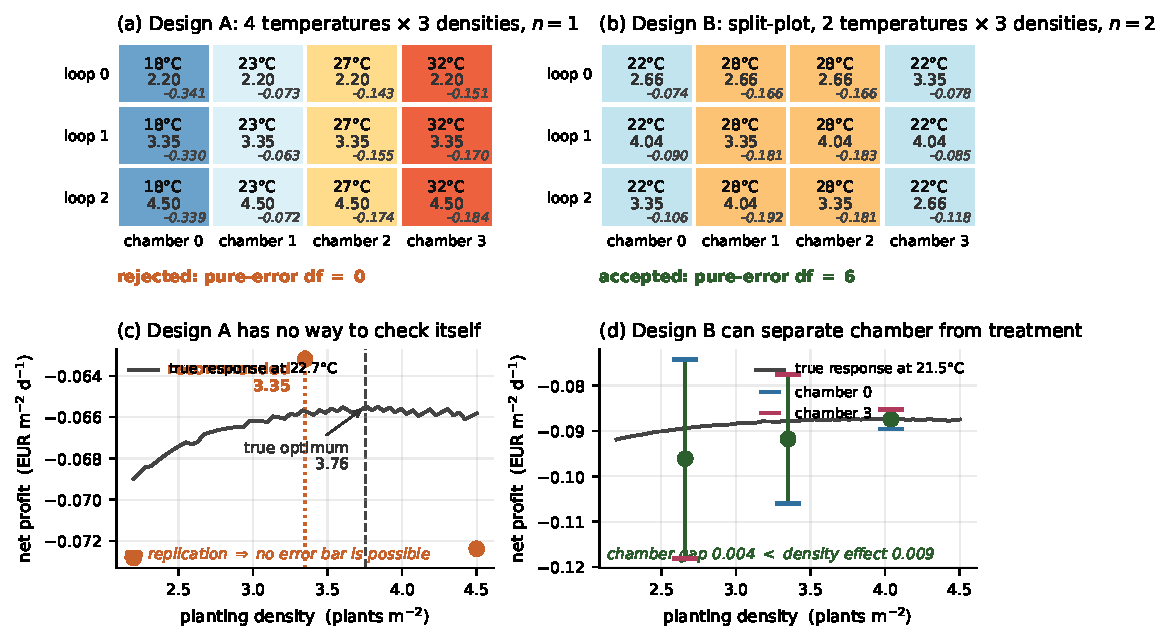
\includegraphics[width=\linewidth]{figures/fig2_worked_example.pdf}
\caption{One round of the running scenario: same site (\texttt{seed=0}), same twelve-unit
budget, two designs. All values are produced by the environment; the script is in the
repository. \textbf{(a)} The intuitive design fills the grid---four temperatures, one per
chamber, crossed with three densities. It passes \texttt{validate\_design}, but every
treatment is observed once, so pure-error df is zero and each temperature is confounded
with one chamber. \textbf{(b)} The split-plot: two temperatures, each replicated across two
non-adjacent chambers, densities randomised within chamber. Our first attempt used chambers
0--1 and 2--3 and was rejected by the randomisation check---temperature then correlates
perfectly with chamber index. \textbf{(c)} Design A's best observation sits at $3.35$ plants\,m$^{-2}$ where the true
optimum at that temperature is $3.76$; the miss is small, and the point is that with one
observation per treatment nothing in the data says whether it is small. \textbf{(d)}
Design B can answer the question it was given: the chamber 0 against chamber 3 gap at
identical settings is $0.004$ against a density effect of $0.009$, so the effect is
resolvable above the block noise --- which is a statement design A cannot make either way.
The figure is regenerated from the frozen environment; an earlier version hard-coded the
annotations and printed the comparison in (d) with the inequality facing the other way.}
\label{fig:worked}
\end{figure}


\section{Task specifications}
\label{app:tasks}

\begin{table}[h]
\centering\small
\begin{tabular}{@{}llll@{}}
\toprule
\textbf{Factor} & \textbf{Range} & \textbf{Control level} & \textbf{Role} \\
\midrule
day temperature   & 18--32\,\textdegree C     & chamber & heating/ventilation setpoint \\
night temperature & 12--22\,\textdegree C     & chamber & setpoint \\
CO$_2$            & 350--1200\,ppm            & chamber & enrichment \\
PAR               & 18--32\,mol\,m$^{-2}$d$^{-1}$ & chamber & natural + supplemental \\
plant density     & 2.2--4.5\,m$^{-2}$        & loop    & planting decision \\
$\mathrm{LAI}_{\max}$ & 2.0--5.0              & loop    & pruning target \\
\bottomrule
\end{tabular}
\caption{The six management factors. Control level is a physical fact---lamps and heating
serve a whole chamber, whereas density and the pruning target are set per hydroponic
loop---and it determines each factor's parallelism ceiling.}
\end{table}

The noise column of Table~\ref{tab:tasks} is
\[
  \sigma_{\mathrm{tot}}/\sqrt{B} \;=\;
  \sqrt{\mathrm{sd}^2\Big(\tfrac{\tau_{\mathrm{loop}}^2}{B}
  + \tfrac{\tau_{\mathrm{chamber}}^2}{CR} + \tfrac{\tau_{\mathrm{batch}}^2}{R}\Big)},
\]
the standard error of the mean of $B = R \times |\mathcal{U}_r|$ observations spread over
$C$ chambers and $R$ rounds. Only the first term falls with $B$: a chamber effect is shared
by every unit in that chamber and a batch effect by every unit in that round, so past a
point buying more units stops buying precision. That is the width constraint of
\S\ref{sec:conditions} in arithmetic.

Two quantities a grower does control are declared by the task rather than exposed as
factors, and the environment refuses to treat either as one. Cycle length is fixed at
$210$ days: it is monotone over any plausible range, because fruit set does not begin until
roughly 30--45 days and that establishment period is pure cost, so exposing it would add a
dimension with the same answer at every site. Leaf removal is fixed at
$2.25$\,g\,node$^{-1}$ because the reduced model gives defoliation no photosynthetic
penalty, so its optimum is always at the upper rail. Both are asserted rather than
silently overridden, so anyone who adds them back gets an error instead of a sweep that
quietly holds them constant.

\section{The naive corner}
\label{app:naive}
Setting every factor to its upper bound yields \emph{negative} profit at every site,
worse than the site optimum by a factor of $4$ to $52$; setting every factor to its
midpoint is also negative at most sites, worse by a factor of $1.3$ to $21$. Maximising everything fails because day temperature at its ceiling aborts fruit set
(eq.~8) while supplemental lighting continues to draw power. We use this rather than
``every factor has an interior optimum'' as the criterion for a non-trivial search problem.

\section{Reproducibility}
\label{app:repro}
All results use seeds $0..N{-}1$; \texttt{SlowLabEnv(task, seed)} is deterministic, and the
seed selects a sampled site rather than only a noise realisation. Every table and figure in this paper is emitted by a script in \texttt{scripts/} from
the JSON under \texttt{results/}, and none is hand-edited. The files carry the environment
version in their names, so a table built from a previous environment cannot be picked up
silently. Code, task definitions and those scripts are released under the MIT licence at
\url{\projecturl}. The $800$ raw language-model transcripts and the cached atom sets are
published there as a release asset rather than in the repository itself.
\todo{datasheet, croissant metadata, hosting}

\section{The $\mathcal{R}^\star$ estimator}
\label{app:eig}

\paragraph{Observation likelihood.} Because the per-unit draw $\phi_u$ is pushed through the
forward model, $p(y \mid \theta, x)$ has no pointwise density. We moment-match the per-unit
response to a Gaussian with variance $s^2(x)$, which makes the covariance of a round's
$|\mathcal{U}_r|$ observations
\[
\Sigma(D_r) \;=\; \operatorname{diag}\!\big(s^2(x_u) + \tau_\gamma^2\big)
\;+\; \tau_\beta^2\, Z Z^{\!\top} \;+\; \tau_\epsilon^2\, \mathbf{1}\mathbf{1}^{\!\top},
\]
with $\tau_\beta, \tau_\gamma, \tau_\epsilon$ the nuisance scales of \S\ref{sec:conditions}
and $Z \in \{0,1\}^{|\mathcal{U}_r| \times C}$ the block-membership matrix. The allocation
enters through $Z$, so where a design places its treatments changes
\eqref{eq:eig}, not only which treatments it chooses.

\paragraph{Three approximations.} \emph{(a)} The Gaussian moment-match above.
\emph{(b)} $s^2(\cdot)$ is computed once at the nominal parameter vector rather than per
atom. \emph{(c)} The prior is the $M$-atom mixture rather than the continuous $P_\Theta$.
We had argued that (c) was benign, on the grounds that the dimension which matters is that
of $x^\star_\theta$ rather than of $\theta$, and that it is small --- over $150$ instances
of \textsc{Optimise} the true optima occupy ten grid cells at
$H\big[p(x^\star_\theta)\big] = 2.05$ nats. That argument is wrong, and the next two
paragraphs are what it cost. The support of $x^\star_\theta$ being small does not make the
\emph{likelihood} over atoms well behaved, and it is the likelihood that fails.
\pending{Moment diagnostics for (a) and (b).}

\paragraph{The in-sample estimator and why we abandoned it.} Our first estimator drew one
atom set and used it for everything: the posterior weights $w_m(y)$, the minimisation over
candidate recommendations, and the evaluation of the chosen recommendation. The failure is
mechanical. $\Sigma(D_r)$ above contains observation noise and block structure and nothing
for the coarseness of the grid, so with $12$ to $24$ observations the likelihood
discriminates between atoms far more sharply than the grid spacing warrants. Measured over
$160$ atoms on \textsc{Optimise}, the mean effective sample size $1/\sum_m w_m^2$ is
$1.1$, and the candidate that minimises $w^{\!\top}\!D$ is some atom's own optimum in
$98\%$ of draws. The estimator was therefore answering ``can the data identify which of
these $160$ sites generated it'' and reporting the answer as though it were ``how much
decision risk does this design remove''. Held out on atoms that did not generate the data,
the same designs score $c = -64\%$ where the in-sample number reads $+97\%$: conditioning on
the design leaves the reasoner worse than the prior-optimal constant, because the posterior
concentrates on a wrong atom and the recommendation follows it there.

\paragraph{The estimator we report.} Three changes, all in
\texttt{achievable\_regret\_cv}. The likelihood is raised to the power $1/T$, equivalently
$\Sigma \to T\Sigma$, which is the minimal way to state that the true site lies between
atoms. $T$ is selected by leave-one-out over the inference atoms: for each atom $m$, draw
$y$ from $m$, form the posterior from the others, choose a recommendation, and score it at
$m$; take the $T$ minimising the average. The evaluation atoms are never touched, so
selecting $T$ cannot import the bias it removes, and the leave-one-out curve tracks the
held-out curve closely enough to be used as its proxy. Finally the recommendation is scored
on the disjoint half. The result is $c$ between $1\%$ and $20\%$ where the in-sample
estimator read $35\%$ to $78\%$, and the orderings differ: on \textsc{Optimise} the
in-sample estimator ranked random search first among the reference strategies and the
repaired one ranks it last.

We tried the obvious cheaper fix first. Fitting the surrogate hyperparameters is not it and
neither is raising $M$ alone; tempering is what moves the number, and the temperature the
calibration selects is $3$ to $100$, meaning the effective observation covariance is one to
two orders of magnitude larger than the noise model alone implies. That is the size of the
discretisation error, stated in the only units available.

\paragraph{Convergence in the atom count.} Table~\ref{tab:conv} runs seven designs at
$M = 80$ and $M = 320$ on the two tasks we could afford at both counts, six runs each. The
designs span the range of $c$ rather than compete: space-filling, a two-level factorial,
four, two and one distinct treatments, and the two degenerate cases of every unit at a
corner and every unit at the centre.

The estimator has not converged and the direction of its error is now the opposite of the
in-sample one. Quadrupling $M$ leaves the degenerate designs where they are and lifts the
good ones: on \textsc{Screen} the space-filling design goes from $0.8\%$ to $16.5\%$. The
reason is the split. At $M = 80$ only $40$ atoms carry the posterior, which is too coarse a
stand-in for $P_\Theta$ for any design to separate, so the measure reports that no design
helps. Every level we report is therefore a lower bound on what a converged estimator would
give, which is the conservative direction for claims of the form ``no agent reaches the
ceiling'' and the awkward one for any claim that a particular agent's design was poor.

Rank correlation between the two counts is $0.82$ on \textsc{Optimise} and $0.64$ on
\textsc{Screen}. That is lower than the in-sample estimator reported and it is the honest
number: the in-sample estimator's near-perfect rank stability was itself an artefact, since
a posterior that always collapses onto one atom is a deterministic function of design
geometry and therefore stable in $M$ for the wrong reason. A single estimate carries a
standard deviation of $2$ to $4$ points. Every $c$ in this paper is a mean over dozens of
designs, where that falls below one point, and the comparisons we draw conclusions from are
paired at fixed $M$.

\begin{table}[h]
\centering\small
\begin{tabular}{@{}lcccc@{}}
\toprule
& \multicolumn{2}{c}{\textsc{Optimise}} & \multicolumn{2}{c}{\textsc{Screen}} \\
\cmidrule(lr){2-3}\cmidrule(lr){4-5}
\textbf{Design} & $c$ at $M{=}80$ & $M{=}320$ & $c$ at $M{=}80$ & $M{=}320$ \\
\midrule
space-filling & $21.7\pm1.3$ & $29.6\pm2.0$ & $0.8\pm0.9$ & $16.5\pm0.8$ \\
four treatments & $2.2\pm1.6$ & $16.0\pm1.4$ & $0.5\pm1.1$ & $7.8\pm0.8$ \\
two treatments & $4.4\pm1.5$ & $12.2\pm1.5$ & $12.9\pm0.9$ & $7.8\pm1.1$ \\
two-level factorial & $-2.0\pm1.8$ & $-0.5\pm2.1$ & $-1.7\pm0.4$ & $3.4\pm1.1$ \\
corner only & $-1.9\pm1.5$ & $-1.7\pm2.1$ & $0.7\pm0.8$ & $1.5\pm0.8$ \\
centre only & $-0.4\pm1.6$ & $-1.9\pm1.7$ & $-0.4\pm1.3$ & $-3.1\pm0.5$ \\
one point & $-2.0\pm1.6$ & $-2.3\pm2.1$ & $-0.7\pm1.1$ & $0.6\pm0.6$ \\
\midrule
\multicolumn{5}{@{}l}{$\mathcal{R}^\star(\varnothing)$: \textsc{Optimise} 0.00546 $\to$ 0.00610; \textsc{Screen} 0.00500 $\to$ 0.00443} \\
\multicolumn{5}{@{}l}{rank correlation of $c$ between the two atom counts: $0.82$ and $0.64$} \\
\bottomrule
\end{tabular}
\caption{Design efficiency at two atom counts under the cross-validated estimator, seven designs chosen to span the range rather than to compete. Each entry is the mean of six independent runs with its standard error; a single run carries a standard deviation of $2$ to $4$ points, which is why the levels reported elsewhere in this paper are always means over dozens of designs. Quadrupling the atom count leaves the two degenerate designs where they were and roughly doubles the best one on \textsc{Optimise}; on \textsc{Screen} it moves the space-filling design from nothing to the top. The estimator is not converged, and the direction of its error at low $M$ is to under-credit good designs, because half of $80$ atoms is too coarse a stand-in for $P_\Theta$ for any design to separate.}
\label{tab:conv}
\end{table}


\paragraph{The bound does not survive estimation.} For the exact quantities $c \in [0,1]$
is a theorem: numerator and denominator start from the same beliefs, so
$\mathbb{E}[\min] \le \min[\mathbb{E}]$ gives $\mathcal{R}^\star(D_r) \le
\mathcal{R}^\star(\varnothing)$, and $\mathcal{R}^\star \ge 0$ closes the other end. The
estimator above is a tempered rule graded out of sample, about which the optimality theorem
says nothing, and the difference is visible: across the $320$ reference rounds behind
Table~\ref{tab:refs}, $69$ carry a negative $c$. Averaged over the dozens of rounds that
make up one cell every value we report is inside $[0,1]$ --- $c$ from $1\%$ to $20\%$,
$\eta$ from $4\%$ to $56\%$ --- but by margin rather than by proof. For $\eta$ there is
not even an exact bound to appeal to, since the agent's $\hat{x}_r$ has seen every round
while the numerator scores each round separately against the prior.

\paragraph{Trajectory and endpoint.} The interim recommendation elicited after each round uses
the same rule the agent applies at the end, so the last point of a trajectory equals the
regret of the submitted recommendation. This is asserted by a regression test: an earlier
version used the best observed point for the trajectory and a posterior maximum for the
submission, which differed by $47\%$ on \textsc{Optimise}.

\section{The horticultural instantiation}
\label{app:domain}

\paragraph{Forward model.} $f_\theta$ is the reduced state-variable TOMGRO model
\citep{jones1999reduced}: five coupled state variables---mainstem nodes, leaf area index,
above-ground, fruit and mature-fruit dry weight---implemented from its equations (1)--(11)
with the published least-squares estimates. We deliberately do not sample ground truth from
a Gaussian-process prior: such a sample has no physical content, its length scale would be
our choice, and it makes the modelling assumption of GP-based agents exactly correct.
Fitting our Bayesian-optimisation reference's own surrogate to the mechanistic response
gives mean absolute error $1.1\times$ the global average in the high-temperature decline and
$2.2\times$ near the kink where supplemental lighting begins to incur cost---real but mild,
and the surrogate still locates the optimum. What the mechanistic surface supplies that a
stationary GP cannot is structure: fruit abortion above $T_\mathrm{CRIT}$ (eq.~8), the
source of irreversibility, and a source--sink limit taking the \emph{minimum} of two growth
expressions (eqs.~9--10). $P_\Theta$ follows the same paper's finding that vegetative
parameters are stable across sites while fruit parameters vary: each seed draws fruit
parameters across the published between-site spread ($N_{FF}$ varies by $2.2\times$ across
their three sites). Five of the six factors have optima that move across sites; the sixth,
supplemental light, sits at the lower rail in every instance because at 2024 European
electricity prices it never repays its energy.

\paragraph{Facility.} Blocks are climate chambers and units are hydroponic loops. Lamps,
heating and CO$_2$ enrichment are set per chamber; planting density, pruning target and
the pruning target is set per loop. Cycle length is fixed at $210$ days for every unit and
is not a decision (\S\ref{sec:tasks}).

\paragraph{Costs.} Revenue is fruit fresh weight at wholesale price; costs are supplemental
lighting, heating and CO$_2$ enrichment, computed with standard greenhouse engineering
relations. Coefficients come from public sources rather than from us, because the
\emph{Costly} measure is denominated in euros and an uncited coefficient makes its absolute
value uninterpretable: crop price 1.50~EUR/kg fresh weight, between Dutch (1.57) and Spanish
(1.35) vine tomato in March 2024 \citep{tomato_prices}; electricity 0.189 and natural gas
0.0605~EUR/kWh, the EU non-household averages for 2024 \citep{eurostat_energy_prices};
luminaire efficacy 2.5\,\textmu mol\,J$^{-1}$, the level over half of listed horticultural
fixtures reach \citep{dlc_qpl}; a cover heat-transfer coefficient of
4.0\,W\,m$^{-2}$K$^{-1}$, between single glass ($\approx$4.5) and double polyethylene
(2.9--3.4) \citep{kittas_covers}. The CO$_2$ leakage coefficient yields 14.6\,kg\,m$^{-2}$
per season, inside the 12--24 range that must be delivered for tomato \citep{ahdb_co2}.

\paragraph{Caveats.} The figures are representative European values, not measurements from
one facility. Outdoor temperatures correspond to the Mediterranean--subtropical winters of
TOMGRO's calibration sites rather than to northern Europe, where greenhouses consume
47--69\,m$^3$ of gas per m$^2$ per year ($\approx$460--670\,kWh) against about 245
here---a difference of climate rather than of coefficients. And one consequence was not our
choice: at these prices supplemental lighting is never economical in this climate, so the
optimum for PAR sits at its lower bound for every site.

\section{Scripted references, and how far they get}
\label{app:refs}

Four scripted strategies ship with the environment: random search over the factor space; a
planned campaign, being a Plackett--Burman screen with centre points followed by a response
surface, replicated and randomised across chambers; and Bayesian optimisation at one and at
two replicates per treatment. Table~\ref{tab:refs} runs all four on all four tasks, eight
instances each. They are a reference point, not a baseline we claim to have tuned: each is
a textbook method implemented straightforwardly, and the numbers below say what such an
implementation achieves at these budgets, not what the method is capable of.

\begin{table}[t]
\centering\small
\begin{tabular}{@{}llcccccc@{}}
\toprule
\textbf{Task} & \textbf{Strategy} & $\bar{\mathcal{R}}(R)\downarrow$ & $\mathcal{R}_{\mathrm{cum}}\downarrow$ & $c\uparrow$ & $\eta\uparrow$ & design & decision \\
 & & final answer & campaign cost & & & rank & rank \\
\midrule
\multicolumn{8}{@{}l}{\textsc{Sanity} \quad \small $\mathcal{R}^\star(\varnothing)=0.0055$} \\
& Random search & 0.0417(119) & 345 & 1\% & 13\% & 3 & 4 \\
& Planned campaign & 0.0089(33) & 140 & 9\% & 56\% & 1 & 1 \\
& Bayesian opt.\ (1 rep) & 0.0172(73) & 289 & 1\% & 32\% & 3 & 3 \\
& Bayesian opt.\ (2 rep) & 0.0128(49) & 288 & 5\% & 41\% & 2 & 2 \\
\addlinespace
\multicolumn{8}{@{}l}{\textsc{Screen} \quad \small $\mathcal{R}^\star(\varnothing)=0.0044$} \\
& Random search & 0.0585(92) & 1061 & 20\% & 6\% & 1 & 1 \\
& Planned campaign & 0.0989(84) & 972 & 5\% & 4\% & 4 & 3 \\
& Bayesian opt.\ (1 rep) & 0.0586(183) & 799 & 16\% & 6\% & 2 & 1 \\
& Bayesian opt.\ (2 rep) & 0.0785(188) & 844 & 12\% & 5\% & 3 & 2 \\
\addlinespace
\multicolumn{8}{@{}l}{\textsc{Optimise} \quad \small $\mathcal{R}^\star(\varnothing)=0.0061$} \\
& Random search & 0.0258(82) & 709 & 3\% & 23\% & 3 & 4 \\
& Planned campaign & 0.0251(98) & 510 & 3\% & 24\% & 3 & 3 \\
& Bayesian opt.\ (1 rep) & 0.0120(37) & 496 & 6\% & 48\% & 1 & 2 \\
& Bayesian opt.\ (2 rep) & 0.0107(37) & 540 & 5\% & 54\% & 2 & 1 \\
\addlinespace
\multicolumn{8}{@{}l}{\textsc{Transfer} \quad \small $\mathcal{R}^\star(\varnothing)=0.0041$} \\
& Random search & 0.0706(51) & 2404 & 17\% & 5\% & 1 & 4 \\
& Planned campaign & 0.0653(81) & 1592 & 8\% & 6\% & 4 & 3 \\
& Bayesian opt.\ (1 rep) & 0.0335(36) & 1418 & 13\% & 11\% & 3 & 1 \\
& Bayesian opt.\ (2 rep) & 0.0534(152) & 1644 & 15\% & 7\% & 2 & 2 \\
\addlinespace
\bottomrule
\end{tabular}
\caption{Reference strategies, environment v1.0.0, eight instances per task. $\bar{\mathcal{R}}(R)$ is the regret of the final recommendation, with its standard error in the last two places; $\mathcal{R}_{\mathrm{cum}}$ is the profit the campaign forwent, in \euro\,per square metre summed over committed unit-days. $c$ is design efficiency against the $\mathcal{R}^\star(\varnothing)$ printed above each block. Rank $1$ is best and tied values share a rank; decision rank orders $\eta$, whose levels are in Appendix~\ref{app:eig}. We draw conclusions from the ranks rather than the levels, for the reason given in \S\ref{sec:estimator}.}
\label{tab:refs}
\end{table}


\paragraph{What is and is not tuned.} The Bayesian-optimisation reference uses a
hand-rolled Gaussian-process surrogate whose length scale and observation noise are fixed
rather than fitted, and the tool arm of \S\ref{sec:results} hands the same routine to a
language model. We assumed the fixed hyper-parameters were costing it and checked
(\texttt{scripts/tool\_hyper\_control.py}): refitting length scale and observation noise by
marginal likelihood on exactly the same observations, holding the recommendation rule and
everything else constant, changes the regret of the point proposed by $-25\%$ on
\textsc{Optimise}, $-6\%$ on \textsc{Screen}, $-5\%$ on \textsc{Transfer} and $+32\%$ on
\textsc{Sanity}: better on three tasks, worse on one, and still several times the regret
the same routine carries when it chooses its own designs. The fixed hyper-parameters are
not what limits either. The planned campaign's screen is full
rank over the factors it varies, which is the only property we checked. Both are released
so that a reader can improve on them.

\paragraph{The two efficiencies come apart on \textsc{Transfer}.} Random search ranks
first on design there and last on decision: it spreads its units over the whole space, so
its observations locate the optimum better than any other strategy's, and it then
recommends close to the best point it happened to run. Bayesian optimisation is the mirror
image, concentrating units near the incumbent and converting far more of what that carries.
On \textsc{Screen} the same pattern holds weakly. It does \emph{not} hold on
\textsc{Optimise}, where the repaired estimator puts all four strategies between $3\%$ and
$6\%$ and the task no longer separates designs at all; the in-sample estimator reported
$39\%$ to $46\%$ there and ranked random search first, and that was an artefact. On
\textsc{Sanity} the planned campaign leads on both, which is what a control should look
like. The stronger demonstration that the two measures are not restatements of each other
is in \S\ref{sec:results}, where one intervention moves them in opposite directions within
a single model.

\paragraph{Where the ratio is thin, nothing converts.} On \textsc{Screen} all four
strategies convert between $4\%$ and $6\%$, so the decision column there is close to two
tied pairs rather than an ordering. This is Table~\ref{tab:tasks}'s ratio of $1.5$
restated: when the room for tailoring is barely above what a full budget resolves, the
difference between a good and a bad reading of the data is not detectable.

\paragraph{A screen presumes a campaign these budgets do not pay for.} On \textsc{Screen}
the planned campaign has the worst realised regret of the four, worse than random search,
although its screening design is full rank over the six factors it varies, replicated and
randomised across chambers. At this budget it spends half its units establishing which
factors matter and the other half on a response surface around a noisy incumbent, while
random search spends everything on coverage. Plackett--Burman was designed for a programme
with a follow-up; two rounds are not one.

\section{How much of the ceiling any design can remove}
\label{app:oracle}

\S\ref{sec:results} reports design efficiency without saying what value of it is
attainable, and a reader is entitled to ask whether a small $c$ measures the agent or the
task. If no admissible design can push $\mathcal{R}^\star(D)$ far below
$\mathcal{R}^\star(\varnothing)$, the denominator of \eqref{eq:capture} carries no
information and a low score says only that the problem is hard.

We answer by searching the admissible set directly
(\texttt{scripts/oracle\_design.py}). The search reads $P_\Theta$ and the forward model, so
it is not an agent and its designs are not achievable by one: it is an upper bound on what
the design half of the score could ever report. The set is discrete and hierarchical ---
chamber-level factors take one value per chamber --- so a round is a choice of how many
chambers, how many loops in each, how many distinct chamber-level and loop-level settings,
and where those settings sit in the factor space. We enumerate that grid over five standard
point families (maximin, Latin hypercube, two-level corners, three-level grid, uniform),
check every candidate through the environment's own validator, and score it with the
cross-validated estimator of \S\ref{sec:estimator}. Being an enumeration over families
rather than a proof of optimality, the $c_{\max}$ of Table~\ref{tab:oracle} is itself a
lower bound on the true maximum.

\begin{table}[h]
\centering\small
\setlength{\tabcolsep}{5pt}
\begin{tabular}{@{}lccccccc@{}}
\toprule
& & \multicolumn{2}{c}{\footnotesize best design found} & \multicolumn{2}{c}{\footnotesize best $c$ achieved} & \multicolumn{2}{c}{\footnotesize median $c$ at} \\
\cmidrule(lr){3-4}\cmidrule(lr){5-6}\cmidrule(lr){7-8}
\textbf{Task} & $\mathcal{R}^\star(\varnothing)$ & $c_{\max}$ & $k$ & model & scripted & $k=2$ & $k \ge d{+}1$ \\
\midrule
\textsc{Sanity}   & 0.0055 & $31.7\%$ & 3 & $11.5\%$ & $9.2\%$  & $1.4\%$ & $5.3\%$ \\
\textsc{Screen}   & 0.0044 & $27.8\%$ & 5 & $7.1\%$  & $20.0\%$ & $2.0\%$ & $10.7\%$ \\
\textsc{Optimise} & 0.0061 & $37.4\%$ & 9 & $18.0\%$ & $5.5\%$  & $9.9\%$ & $15.6\%$ \\
\textsc{Transfer} & 0.0041 & $26.5\%$ & 8 & $9.2\%$  & $16.8\%$ & $4.6\%$ & $12.5\%$ \\
\bottomrule
\end{tabular}
\caption{What one round of design can buy. $c_{\max}$ is the highest design efficiency
found over the admissible set, and $k$ the number of distinct treatments the design
carrying it uses. The next two columns are the best $c$ any language model and any scripted
strategy reached on that task. The last two are the \emph{median} $c$ over all candidates
with two distinct treatments and over all candidates with at least $d+1$, which is the
comparison the diagnosis in \S\ref{sec:results:design} rests on.}
\label{tab:oracle}
\end{table}

Three readings. First, \textbf{the ceiling is not approachable}: the best design found
removes $27\%$ to $37\%$ of $\mathcal{R}^\star(\varnothing)$, so most of the no-data risk
survives any single round at these budgets. That is a property of the regime rather than of
the agents --- twelve to twenty-four units against a six-dimensional site distribution
cannot identify the optimum --- and it is a second reason, beyond the estimator's
convergence, to read $c$ as a rank rather than as a fraction captured.

Second, \textbf{the headroom over what agents reach is real}. The best $c$ anyone achieves
is $1.4\times$ to $2.8\times$ below $c_{\max}$ on every task, so the low values in
Table~\ref{tab:results} are not the measure bottoming out.

Third, \textbf{the width diagnosis survives its own counterexample}. The best design we find
on \textsc{Screen} uses five distinct treatments over six factors, so it is rank-deficient
by the criterion of \S\ref{sec:results:design}: a well-placed narrow design can do well.
But the median tells the other story --- at $k=2$ the median candidate captures $1.4\%$ to
$9.9\%$ depending on the task, against $5.3\%$ to $15.6\%$ at $k \ge d+1$, and the ordering
holds on all four. An agent choosing a narrow design is choosing from that distribution
without being able to see the surface in advance, and the agents' realised $c$ sits close to
the narrow median rather than to its best case.

\section{Does the ordering replicate?}
\label{app:stability}

Two tasks have a prize no larger than the noise a full budget leaves behind
(Table~\ref{tab:tasks}: the ratio is $0.8$ on \textsc{Screen} and $1.0$ on
\textsc{Transfer}), which invites the objection that any ordering they produce is a coin
toss. We measure it (\texttt{scripts/rank\_stability.py}). The twenty instances are split
into two disjoint halves of ten, the five models are ranked on each half by mean realised
regret, and the two rankings are correlated; every model sees the same sites within a half,
so the only thing varying is which sites were drawn. Over $4000$ random splits:

\begin{table}[h]
\centering\small
\begin{tabular}{@{}lcccc@{}}
\toprule
\textbf{Task} & ratio (Table~\ref{tab:tasks}) & $\rho$ between halves & $P(\rho > 0)$ & same winner \\
\midrule
\textsc{Screen}   & 0.8 & $-0.28$ & $0.27$ & $0.09$ \\
\textsc{Transfer} & 1.0 & $+0.09$ & $0.54$ & $0.23$ \\
\textsc{Sanity}   & 1.3 & $+0.40$ & $0.83$ & $0.42$ \\
\textsc{Optimise} & 2.2 & $+0.76$ & $1.00$ & $0.12$ \\
\bottomrule
\end{tabular}
\caption{Split-half stability of the five-model ordering by realised regret, bare arms,
ordered by the ratio of Table~\ref{tab:tasks}. \emph{same winner} is how often the
best-ranked model agrees between halves.}
\label{tab:stability}
\end{table}

The ratio predicts the answer exactly: in Table~\ref{tab:stability} the four tasks fall in
the same order on both columns. At these sample sizes only \textsc{Optimise} produces a per-model ordering that
replicates; \textsc{Screen}'s anti-correlates and \textsc{Transfer}'s is indistinguishable
from zero. The design and decision efficiencies behave the same way ($c$ at $-0.13$,
$+0.55$, $+0.36$ and $+0.74$ in the same task order), which is expected, since they are
computed on the same twenty draws.

This bounds what \S\ref{sec:results} may claim. Every finding there that names an
individual model on \textsc{Screen} or \textsc{Transfer} is under-powered, and we do not
make one. What the section does claim is of three other kinds, none of which ranks models:
proportions of submitted designs, which do not involve the outcome at all; within-model
contrasts paired by site and tested as such, which is how the tool arm is read; and
statements that hold in every cell rather than in a particular order among them. Raising
the instance count is the obvious remedy, and the cost is linear in it: twenty sites times
four tasks times ten arms is already $800$ episodes.

\section{Pricing the irreversibility axis}
\label{app:irrev}

Three of the four conditions have no dial in this domain: a growing cycle takes as long as
it takes, plant-to-plant variation is what it is, and a crop grown is a crop sold. The
fourth has one. Commitment is irreversible throughout --- a submitted design cannot be
revised and the units it occupies are gone for a cycle --- but beyond commitment the
environment implements damage: fruit abortion above $T_{\mathrm{CRIT}}$ puts a unit into a
recovery period graded by how far the threshold was exceeded, so a badly chosen treatment
costs capacity in the \emph{following} round and not only in its own. The four tasks ship
with that recovery length set to zero, so every number in the main tables is at zero. This
appendix turns it up, which is what makes ``the four conditions matter jointly'' a
measurement rather than a claim about the domain.

It is not dead code for want of triggering: across the reference strategies $55\%$ to
$60\%$ of committed units exceed the threshold, by $4.3$ to $4.6\,^\circ$C on average.

\paragraph{Scripted references.} Each of the four is run on each
task at recovery lengths of zero, sixty and two hundred and ten days, twenty instances
each, identical in every other respect and paired by site
(\texttt{scripts/} \texttt{recovery\_sweep.py}). The dial bites: at sixty days
every episode but one of the $320$ loses capacity, and the cell means run from $78$ to
$1071$ unit-days, $2\%$ to $12\%$ of what the campaign used; at two hundred and ten they run
from $272$ to $3747$, $8\%$ to $42\%$. Realised regret moves by $-10\%$ to $+20\%$ and
\emph{not one of the sixteen cells moves by as much as two standard errors of its own
paired difference}. The two non-zero settings are also indistinguishable from each other,
in every cell to four digits, because the blocking granularity is a round: both remove the
unit from exactly one.

\paragraph{Language models.} That measurement has a boundary: none of the four references
replans around lost capacity,
since each constructs its design from the task rather than from what the facility can still
run, so it prices the loss of units to an agent that ignores it. A language model does see
the shortened \texttt{available\_units} list and can respond, so we ran that arm too
(\texttt{scripts/recovery\_llm.py}): five models on \textsc{Optimise}, the same twenty
sites, bare interface, $210$ days against the $0$ of the main tables, one hundred paired
episodes. The dial reaches the agents --- the rounds they submit shrink by $27\%$ and
$23\%$ in the second and third rounds, and infeasible submissions per episode rise from
$0.70$ to $1.22$ as models keep asking for units the facility no longer has. Realised
regret again does not move: $0.0230$ against $0.0221$, a paired $t$ of $-0.34$ at
$p = 0.74$, worse in fifty-one of the hundred. Per-model differences run from $-33\%$ to
$+44\%$ with one at $p = 0.02$, but at a sampling temperature of $0.7$ a rerun at the same
setting would move a twenty-instance cell by about as much (Appendix~\ref{app:stability}),
so only the pooled test is worth reading.

Both halves say the same thing, and it refines the claim rather than supporting it. At
these budgets extra units buy nothing, so losing them costs nothing; what binds is the
number of cycles and the width of the design, not the number of slots. Irreversibility in
v1.0 therefore acts through \emph{commitment} --- a design cannot be revised and a cycle is
spent either way --- and not through the loss of capacity, even when a quarter of the
facility is withdrawn. A version that wanted capacity loss to bite would have to make
replication pay first.

\section{Known defects, and why we stopped fixing them}
\label{app:defects}

The environment is frozen at v1.0. This register is complete as far as we know it, and we
do not intend to fix all of it. A benchmark is a fixed artefact; its value is comparability
across agents, not correctness of the simulator.

\paragraph{The stopping rule.} \emph{A defect is fixed if it changes a claim the paper
makes, and recorded if it does not.} We adopted this after the alternative became visible:
while $\mathcal{R}^\star(\varnothing)$ was being used as an admission test for tasks, every
correction to the crop or cost model moved the ceiling, which moved the task set, which
motivated the next correction. That loop does not terminate, because a simulator can always
be made more nearly right. Reporting ranks rather than levels (\S\ref{sec:estimator}) removes the
dependence and lets the rule bite.

\paragraph{The rule caught four defects and let three stand.} Four defects changed claims and
were fixed: a weight $\lambda$ on the cost term, nominally a task-design parameter, which
set where every optimum sat and pushed four of six factors onto their rails at
$\lambda=0.25$; a photosynthesis routine that read global nominal parameters instead of the
site's, so that every site had an identical light and CO$_2$ response and a stated
limitation about sampling those parameters was a no-op; a heating model that applied
$A\,U\,\Delta T$, the peak-sizing formula for the coldest night, to all $24$ hours of $210$
days, overstating a term worth $48\%$ of variable cost; and an objective named net profit
that omitted harvest labour, grading loss and all fixed costs. One defect was recorded
instead: the block effects below, which affect only the ratio in Table~\ref{tab:tasks}, and
that ratio is no longer a gate.

\paragraph{Noise model.} The block scales $\tau_{\mathrm{chamber}}$,
$\tau_{\mathrm{loop}}$ and $\tau_{\mathrm{batch}}$ multiply the standard deviation of the
objective over uniformly random points in the whole factor space, a quantity dominated by
corners no grower would operate in. Improving the ventilation physics left the optimum
unmoved to three figures and inflated that standard deviation by $71\%$, and with it the
chamber effect, from $4.4\%$ to $7.9\%$ of revenue at the optimum. A chamber's climate
uniformity has nothing to do with how bad the worst corner of the design space is; the
effect should be a temperature offset pushed through the forward model, with a magnitude
taken from measured greenhouse uniformity. Separately, \texttt{task.noise\_sd} is a declared
value $1.3$ to $1.9$ times the per-unit standard deviation the simulator actually produces;
the simulator is right and the declared value is unused except in reporting.

\paragraph{Crop and cost model.} The profit-optimal yield averages
$28$\,kg\,m$^{-2}$yr$^{-1}$ over sites, range $21$ to $37$, against a commercial
$50$--$70$, while the model's \emph{maximum attainable} yield is $59$, inside that range:
the model can grow a commercial crop and does not think it pays. We have not established
why. Supplemental light is rail-bound at every site, so the entire lighting
sub-model has zero elasticity on the objective. This is also what lowers the
\textsc{Screen} ceiling, and it separates two questions a sensitivity analysis conflates:
over $24$ sites, setting supplemental light mid-range rather than at its optimum costs
$0.080$, the largest of the six factors, while setting it at the across-site mean optimum
--- all an experiment could still recover --- costs $0.000$, because its optimum does not
move. The factors worth an experiment are day temperature and CO$_2$, at $0.0085$ and
$0.0060$, together $85\%$ of what instance-tailoring can recover there
(\texttt{scripts/factor\_value.py}). Relatedly, $\mathrm{par}_{\mathrm{ambient}}$ is
fixed across sites although natural daily light integral is the largest real difference
between a Dutch and an Almerian greenhouse. A daily-timestep model cannot represent a
time-varying CO$_2$ enrichment strategy, which is what growers actually run. The
ventilation capacity is clipped rather than allowed to fail, so overheating above that cap
is not modelled.

\paragraph{Provenance of coefficients.} Electricity and gas prices, the site-level spreads,
the LED efficacy range and the cover heat-transfer range are cited. Four numbers are not:
the tomato price, whose source we can no longer verify and which carries the largest
elasticity on the objective; the fruit dry-matter fraction, which has no citation at all and
carries the second largest; the transplant cost, quoted in dollars and used as euros; and
two labour coefficients whose derivations contain wage and task-share figures that are ours.
One property limits the damage: the tomato price and the dry-matter fraction scale revenue
linearly and $\mathcal{R}^\star$ scales with them, so they cancel from every ratio we
report. $\mathcal{R}^\star(\varnothing)$ is $3.1\%$ of revenue at the optimum on both
\textsc{Sanity} and \textsc{Optimise}, and adding harvest labour and grading loss left
that ratio where it was. These coefficients set the euro scale and no conclusion.

\paragraph{Estimator and action space.} The estimator's own defects, and the one we found
and repaired, are in Appendix~\ref{app:eig}; they are the largest single item in this
register. Separately, replication does not pay at these budgets, so an agent is never
rewarded for buying precision --- an arithmetic consequence of bounded parallelism rather
than a bug, but it narrows what the benchmark can distinguish.

\paragraph{A stronger form of irreversibility is implemented and not enabled.} All four
tasks set the recovery length to zero, with the comment ``0 = off (default, keeps existing
results unchanged)'' --- which is the reasoning this appendix opens by arguing against, and
we record it as such rather than defend it. Appendix~\ref{app:irrev} turns it on and
reports what changes.

\paragraph{Two actions a real grower has and this agent does not.} The action space stops
at a design and a recommendation, and two of the omissions matter more than the rest.

\emph{Early termination.} A greenhouse is watched continuously---climate at minute
resolution, crop registration weekly, harvest accumulating from about week ten---so a grower
who has planted a bad treatment usually knows by week six and pulls it. We have no such
action: a committed unit runs its full $210$ days. The omission is what makes \S\ref{sec:regime}'s
two readings of delay, information and action, coincide here; restoring it would separate
them, and it is the cleanest available trade-off between slowness and irreversibility,
since salvaging costs part of a season rather than all of it.

\emph{Staggered planting.} Rounds are synchronous: every unit in a round starts and ends
together. Real trial programmes run a pipeline, starting a new batch every few weeks. Our
budgets leave half the facility idle on two of the four tasks---$8$ of $16$ unit-slots on
\textsc{Sanity} and $12$ of $24$ on \textsc{Screen}---for the full $420$ days, which no
grower would accept. Staggering at a $105$-day offset would run four batches instead of two
in the same wall-clock. It also poses the harder question: with only partial information
from batch one, what do you plant in batch two? That is where slow feedback actually bites,
and it is the first thing we would add.

An agent also cannot choose what to measure, when to measure it, or how many plants to grow
per unit.


\end{document}
